\documentclass[10pt,a4paper,conference]{IEEEtran}

% Some very useful LaTeX packages include:
% (uncomment the ones you want to load)

% *** CITATION PACKAGES ***
%
\ifCLASSOPTIONcompsoc
  % IEEE Computer Society needs nocompress option
  % requires cite.sty v4.0 or later (November 2003)
  \usepackage[nocompress]{cite}
\else
  % normal IEEE
  \usepackage{cite}
\fi
% cite.sty was written by Donald Arseneau
% V1.6 and later of IEEEtran pre-defines the format of the cite.sty package
% \cite{} output to follow that of IEEE. Loading the cite package will
% result in citation numbers being automatically sorted and properly
% "compressed/ranged". e.g., [1], [9], [2], [7], [5], [6] without using
% cite.sty will become [1], [2], [5]--[7], [9] using cite.sty. cite.sty's
% \cite will automatically add leading space, if needed. Use cite.sty's
% noadjust option (cite.sty V3.8 and later) if you want to turn this off.
% cite.sty is already installed on most LaTeX systems. Be sure and use
% version 4.0 (2003-05-27) and later if using hyperref.sty. cite.sty does
% not currently provide for hyperlinked citations.
% The latest version can be obtained at:
% http://www.ctan.org/tex-archive/macros/latex/contrib/cite/
% The documentation is contained in the cite.sty file itself.
%
% Note that some packages require special options to format as the Computer
% Society requires. In particular, Computer Society  papers do not use
% compressed citation ranges as is done in typical IEEE papers
% (e.g., [1]-[4]). Instead, they list every citation separately in order
% (e.g., [1], [2], [3], [4]). To get the latter we need to load the cite
% package with the nocompress option which is supported by cite.sty v4.0
% and later. Note also the use of a CLASSOPTION conditional provided by
% IEEEtran.cls V1.7 and later.


% *** GRAPHICS RELATED PACKAGES ***
%
  \usepackage[pdftex]{graphicx}
  \graphicspath{{../Figures/}}
  \DeclareGraphicsExtensions{.pdf,.png}
  \usepackage{color}

% *** MATH PACKAGES ***
%
\usepackage[cmex10]{amsmath}
% A popular package from the American Mathematical Society that provides
% many useful and powerful commands for dealing with mathematics. If using
% it, be sure to load this package with the cmex10 option to ensure that
% only type 1 fonts will utilized at all point sizes. Without this option,
% it is possible that some math symbols, particularly those within
% footnotes, will be rendered in bitmap form which will result in a
% document that can not be IEEE Xplore compliant!
%
% Also, note that the amsmath package sets \interdisplaylinepenalty to 10000
% thus preventing page breaks from occurring within multiline equations. Use:
%\interdisplaylinepenalty=2500
% after loading amsmath to restore such page breaks as IEEEtran.cls normally
% does. amsmath.sty is already installed on most LaTeX systems. The latest
% version and documentation can be obtained at:
% http://www.ctan.org/tex-archive/macros/latex/required/amslatex/math/

%\usepackage{amssymb}%............................ AMS Symbol fonts



% *** SPECIALIZED LIST PACKAGES ***
%
%\usepackage{algorithmic}
% algorithmic.sty was written by Peter Williams and Rogerio Brito.
% This package provides an algorithmic environment for describing algorithms.
% You can use the algorithmic environment in-text or within a figure
% environment to provide for a floating algorithm. Do NOT use the algorithm
% floating environment provided by algorithm.sty (by the same authors) or
% algorithm2e.sty (by Christophe Fiorio) as IEEE does not use dedicated
% algorithm float types and packages that provide these will not provide
% correct IEEE style captions. The latest version and documentation of
% algorithmic.sty can be obtained at:
% http://www.ctan.org/tex-archive/macros/latex/contrib/algorithms/
% There is also a support site at:
% http://algorithms.berlios.de/index.html
% Also of interest may be the (relatively newer and more customizable)
% algorithmicx.sty package by Szasz Janos:
% http://www.ctan.org/tex-archive/macros/latex/contrib/algorithmicx/

% *** ALIGNMENT PACKAGES ***
%
\usepackage{array}
% Frank Mittelbach's and David Carlisle's array.sty patches and improves
% the standard LaTeX2e array and tabular environments to provide better
% appearance and additional user controls. As the default LaTeX2e table
% generation code is lacking to the point of almost being broken with
% respect to the quality of the end results, all users are strongly
% advised to use an enhanced (at the very least that provided by array.sty)
% set of table tools. array.sty is already installed on most systems. The
% latest version and documentation can be obtained at:
% http://www.ctan.org/tex-archive/macros/latex/required/tools/


\usepackage{mdwmath}
\usepackage{mdwtab}
% Also highly recommended is Mark Wooding's extremely powerful MDW tools,
% especially mdwmath.sty and mdwtab.sty which are used to format equations
% and tables, respectively. The MDWtools set is already installed on most
% LaTeX systems. The lastest version and documentation is available at:
% http://www.ctan.org/tex-archive/macros/latex/contrib/mdwtools/

% IEEEtran contains the IEEEeqnarray family of commands that can be used to
% generate multiline equations as well as matrices, tables, etc., of high
% quality.

% *** SUBFIGURE PACKAGES ***
\ifCLASSOPTIONcompsoc
  \usepackage[caption=false,font=normalsize,labelfont=sf,textfont=sf]{subfig}
\else
  \usepackage[caption=false,font=footnotesize]{subfig}
\fi

%Setting captions to centered (Not IEEE journal standard)
%\makeatletter
%\long\def\@makecaption#1#2{\ifx\@captype\@IEEEtablestring%
%\footnotesize\begin{center}{\normalfont\footnotesize #1}\\
%{\normalfont\footnotesize\scshape #2}\end{center}%
%\@IEEEtablecaptionsepspace
%\else
%\@IEEEfigurecaptionsepspace
%\setbox\@tempboxa\hbox{\normalfont\footnotesize {#1.}~~ #2}%
%\ifdim \wd\@tempboxa >\hsize%
%\setbox\@tempboxa\hbox{\normalfont\footnotesize {#1.}~~ }%
%\parbox[t]{\hsize}{\normalfont\footnotesize \noindent\unhbox\@tempboxa#2}%
%\else
%\hbox to\hsize{\normalfont\footnotesize\hfil\box\@tempboxa\hfil}\fi\fi}
%\makeatother


% *** FLOAT PACKAGES ***
%
\usepackage{fixltx2e}
% fixltx2e, the successor to the earlier fix2col.sty, was written by
% Frank Mittelbach and David Carlisle. This package corrects a few problems
% in the LaTeX2e kernel, the most notable of which is that in current
% LaTeX2e releases, the ordering of single and double column floats is not
% guaranteed to be preserved. Thus, an unpatched LaTeX2e can allow a
% single column figure to be placed prior to an earlier double column
% figure. The latest version and documentation can be found at:
% http://www.ctan.org/tex-archive/macros/latex/base/

% *** PDF, URL AND HYPERLINK PACKAGES ***
%
\usepackage{url}

\usepackage{sistyle}
    \SIstyle{S-Africa}
    \SIunitspace{{\cdot}}
    \SIunitdot{{\cdot}}

% generate nice bookmarks and hyperrefs when exporting to pdf and dvi (screen version):
\usepackage[a4paper,plainpages=false,colorlinks,linktocpage,bookmarks=true,bookmarksopen=false]{hyperref}
% use this for printing only (no color, print version):
%\usepackage[a4paper,plainpages=false,colorlinks=false,linktocpage,bookmarks=true,bookmarksopen=false]{hyperref}

% correct bad hyphenation here
\hyphenation{op-tical net-works semi-conduc-tor}

%Add elegant support for Big-O notation
\providecommand{\OO}[1]{\operatorname{O}\left(#1\right)}

\begin{document}

%
% paper title
\title{Pithos: A Hybrid Multi-Tiered State Persistency Architecture for Peer-to-Peer Massively Multiuser Virtual Environments}

%\author{\IEEEauthorblockN{John S. Gilmore and Herman A. Engelbrecht\\}
%\IEEEauthorblockA{MIH Media Lab\\
%Electronic Engineering Department\\
%Stellenbosch University\\
%Stellenbosch, South Africa\\
%mail: jgilmore@ml.sun.ac.za and hebrecht@sun.ac.za}}

\maketitle

\begin{abstract}
%\boldmath
The abstract goes here

\end{abstract}


\section{Introduction}
\label{introduction}

%
% Admittedly, this is a hack and may well be fragile, but seems to do the
% trick for me. Note the need to keep any \label that may be used right
% after \section in the above as the hack puts \section within a raised box.

% The very first letter is a 2 line initial drop letter followed
% by the rest of the first word in caps (small caps for compsoc).
%
% form to use if the first word consists of a single letter:
% \IEEEPARstart{A}{demo} file is ....
%
% form to use if you need the single drop letter followed by
% normal text (unknown if ever used by IEEE):
% \IEEEPARstart{A}{}demo file is ....
%
% Some journals put the first two words in caps:
% \IEEEPARstart{T}{his demo} file is ....
%

%P2P MMVE Background
\IEEEPARstart{P}{eer-to-Peer (P2P)} Massively Multiuser Virtual Environments (MMVEs) have received significant attention from the research community,
since the first publication on the subject by Knutssonn et al. in 2004 \cite{knutsson_p2p_first}. P2P MMVEs promise to solve many issues prevalent in
today's Client/Server (C/S) based MMVEs. Some key issues have to be solved before P2P MMVEs can be implemented commercially. Over the past few years,
researchers have been addressing these challenges.

%Key challenges and focus
Recently, six key challenges of P2P systems have been identified: Interest Management, Game Event Dissemination, Non-player Character (NPC) Host
Allocation, Game State Persistency, Cheating Mitigation and Incentive Mechanisms \cite{Fan_deisgn_issues_p2p}. Most of the challenges mentioned have
received significant attention from the research community, except for state persistency.

State persistency defines how object states should be stored. This allows for storing anything from a user's position to the state of the virtual
market in an MMVE. For a P2P MMVE, game data must be distributed amongst various peers in the network. This creates challenges not usually present in
classic C/S MMVEs. The focus of this paper is exclusively on state persistency in P2P MMVEs.

%Current techniques not perfect
The paper first attempts to group state persistency mechanisms found in the literature. The paper then shows that none of the approaches to state
persistency has thus far been sufficient to meet the storage requirements of MMVEs of today. All storage models are evaluated according to the
identified requirements of scalability, fairness, reliability, responsiveness and security.

%Propose multi-tiered model
Because current state persistency models do not address all the requirements of modern MMVEs, a novel hybrid multi-tiered state persistency model is
proposed, called Pithos, that is based on grouping players in some logical way and allowing for responsive interaction between players in the same
group, with lower levels of responsiveness between groups. The supposition is that players have more interest in other object and player states close
to them than far from them.

%Implementation
The proposed multi-tiered model is currently being implemented in Oversim, a peer-to-peer simulation environment based in Omnet++. The model allows
for the measurement of the requirements of scalability, fairness, reliability and responsiveness. Furthermore, it allows for the comparison of the
current model with other state persistency models. Initial results seem promising, with the implemented model functioning as expected. The system
shows to be very responsive when storing data within a group and as responsive as storing data in an overlay when storing data between groups.

%Summary
Section \ref{current_models} groups storage models found in the literature and describes the advantages and disadvantages of each group. The section
concludes with a comparison of the different storage models and comments on their applicability to P2P MMVEs.
%
Section \ref{proposed_model} introduces our proposed state persistency model and describes the different assumptions on which it is based.
%
Section \ref{implementation} describes the implementation details of the proposed model.
%
Section \ref{results} presents some preliminary results.
%
Section \ref{conclusion} concludes with a summary of the paper and a discussion on possible future work.

\section{Distributed state persistency models}
\label{current_models}

%Overview of four approaches
Four approaches have been identified by which state persistency is achieved in P2P MMVEs. These are: \emph{super peer storage}, \emph{overlay
storage}, \emph{distance-based storage} and \emph{hybrid storage}. Requirements have also been identified by which storage systems should be
measured. These are: scalability, fairness, reliability, responsiveness and security.

%Scalability
For an MMVE state persistency architecture to be scalable, it should be able to support large, typically thousands of users. In the paper,
scalability it not handled as some separate entity, but rather all other requirements are evaluated in terms of a system of thousands of users.
%Reliability
Reliability is defined to mean that a file in the storage system may neither be lost, nor not be available when a user requests it.
%Fairness
For a system to be fair, the responsibility of storage should be equally shared amongst all users. Ideally, a fair scheme should take the
heterogeneity of peers into account. This ensures that costs due to bandwidth and storage are shared amongst all users.
%Responsiveness
Responsiveness is a requirement that has not really been part of file storage systems in the past. Usually, it doesn't matter much how low it takes
to resolve a file storage or request, just that the file is stored or retrieved. Sizes of files are usually large and so the time storage and
retrieval operations take are usually constrained by the available bandwidth. For games, it is believed that responsive object storage is a key
requirement to promote responsive gameplay and robust recovery mechanisms. Especially because it is expected that game objects are in general much
smaller than the files, which normal storage systems are designed for.
%Security
Data security is a major issue for distributed storage, because data are stored on users' machines who should not necessarily be able to access and
alter the data stored.

To clarify what type of objects are stored in these types, only the root objects, also called the authoritive objects, are considered for storage. It
is still assumed that replica objects that are used by players to render the world are locally stored and that these objects derive their states from
the respective root objects.

\begin{table*}[htbp]
\centering
\begin{tabular}{|r|c|c|c|c|}
\hline
Storage type & Reliability & Responsiveness & Security & Fairness\\
\hline
Super Peer & Medium & High & Low & Low\\
Overlay & High & Low & Medium & High\\
Hybrid & High & High & Medium & Low\\
Distance-based & Medium & High & Low & Medium\\
\hline
\end{tabular}
\caption{Differences between storage mechanisms} \label{tab_storage}
\end{table*}
%
Table \ref{tab_storage} presents a characterisation of current storage systems according to the characteristics defined. Table \ref{tab_storage} also
provides some references that act as examples of the different storage types mentioned. These example architectures will be discussed briefly in the
sections to follow.

\subsection{Super peer storage}

%Super peer storage - description
Super peer storage relies on the super peer storing all information that is in its domain \cite{knutsson_p2p_first}. A domain is usually created by
segmenting the world into regions and super peers act as regional servers to all peers in their region. Each super peer handles state persistency for
its region, hosting NPCs, objects and persistent player data. This storage method is much like a Client/Server setup, with the super peer acting as
the server for the virtual geographic region assigned to it.

The advantage of super peer storage is that it's fairly simple to implement using well known database solutions.

The disadvantages of super peer storage stem from the per-region centralised approach. It is difficult to achieve high levels of reliability, without
some migration mechanism that requires redundant super peers per region and allows for migration of data and responsibilities when a super peer
leaves the network. Because super peers are merely users in the virtual world, they can be expected to regularly join and leave the world. It is
possible to implement such mechanisms, although that would significantly complicate the implementation task. No current architectures are known to
have implemented such a mechanism so the difficulties associated with this approach have not been explored.

The main issues with super peer storage are those of fairness and security. Because a single super peer controls all data in a region and because
that super peer is merely another user, there might be a high possibility that the data can be compromised in some way. There is also a high
incentive to be able to modify data in a region by a user operating in that region. It is also difficult to secure the data, because any user should
have access to, for example, another user's position. If the super peer user can identify which data is which, he might be able to modify that data.

Fairness is another issue with super peer storage, because the super peers are expected to store all the region data and are also expected to donate
their bandwidth to service requests for data from all region peers.


\subsection{Overlay storage}

%Description
Overlay storage is classified as using any type of structured P2P overlay to store data in a distributed fashion \cite{Douglas05enablingmassively},
\cite{using_freenet_storage}, \cite{Fan_phd}, \cite{past_storage_focus}. This is a very broad definition, which basically encompasses any P2P
distributed storage currently in use. Some examples and a comparison of different distributed storage techniques can be found in
\cite{Hasan_distributed_storage_survey}. The reasoning is that any P2P distributed storage can be used to only store game files. Therefore,
distributed storage is used as a distributed database for game files.

%Advantages/Disadvantages
The main advantages of overlay storage is its reliability and fairness. Because data are distributed across all nodes, overlay storage is the fairest
storage system reviewed. Because data are hosted by many nodes, redundancy may be used to make the system reliable. Because of the distance based
routing mechanism used in most P2P overlays, redundancy is easily implemented by placing replica data at a node's overlay neighbours. Overlay storage
can also be made reasonably secure, because it is possible to leverage the redundancy mentioned and multiple routing paths present in the overlay.

The main disadvantage of overlay storage is responsiveness. The routing time in overlay storage is of order $O(\log(N))$, where N is the total number
of nodes in the network. This can be considered an efficient routing time in general, but for real-time applications that require real-time access to
data, this routing complexity is not considered ideal.

\subsection{Hybrid storage}

%Description
The world is divided into regions, with each region controlled by a super peer \cite{zoned_federation}, \cite{hybrid_storage1}. The complete region
state is cached at every super peer, the same as with super peer storage. There also exists a backup overlay storage architecture, to which data may
be backed up for long term, redundant and secure storage. The hybrid region-based overlay storage contains many improvements over pure overlay
storage as will be discussed in the following sections.

%Advantages/Disadvantages
Hybrid storage combines some of the features present in overlay and super peer storage to have the advantages of high reliability and responsiveness.
Reliability is achieved from redundancy present in overlay storage and responsiveness is achieved by the direct access peers have to their respective
super peer.

Hybrid storage still partly suffers from the security issues present in super peer storage, but overlay storage allows for replication which creates
reference objects to which the super peer objects might be compared. Checking every super peer object against the corresponding overlay object will,
however negate any advantages received from super peer storage in terms of responsiveness.

Hybrid storage still suffers from the lack of fairness present in super peer storage. Although data are distributed amongst all nodes for overlay
storage, there still exists super peer nodes that also possess all data present in the network, making the storage almost as unfair as super peer
storage.

\subsection{Distance-based storage}
\label{classic_distance_based}

%Description
Distance based approaches, such as the Voronoi storage approaches \cite{Buyukkaya_voronoi_state_management}, \cite{Hu_voronoi_IM} and some more
general approaches \cite{colyseus_distance_based}, \cite{solipsis}, store object data on the peer closest to the object in the virtual world. Some
distance metric is used to determine on which node an object should be stored. In some systems, only player states are considered for storage
\cite{individual_storage1}, \cite{cheat_proof_playout}. This storage is termed individual storage and is considered as a subset of distance storage,
which also allows for non-player objects to be stored.

%Advantages/Disadvantages
Responsiveness is considered to be the main advantage of distance-based storage. It is considered that the player that is close to an object has more
interest in that object than a player that is far away. This means that the player with the most interest in an object will be most likely to be
locally hosting that object. This is not always the case, but for cases where the player hosting the object has to serve that object to another
player, the system is still as responsive as super peer and normal C/S-based storage. Distance-based storage can also be made reliable by
implementing some replication and migration mechanisms or implementing it as a distance-based overlay storage hybrid. Such implementation have not
been presented in the literature reviewed.

Two issues with distance-based storage are security, and to a lesser degree, fairness. Security is a major concern, since data are by design, stored
on nodes with the most interest in it. This means that a node that stores data has the most interest to be able to modify that data in contravention
of the virtual environment rules. Although all nodes share all objects in the virtual world, some nodes might have to store more data than others
depending on user density in the virtual world and on how many objects are close to the different nodes.

\subsection{Summary and comparison}

From this discussion, it is evident that none of the mentioned storage types in their current forms are appropriate for data storage in MMVEs. None
of the storage types meet all the requirements as set out. Super peer storage is not fair or secure, overlay storage is not responsive, hybrid
overlay/super peer storage is not fair and distance-based storage is not secure and not yet reliable.

It should also be noted that most of these storage types are not mature. In the referenced papers, they were mentioned as a means by which
persistency might be achieved. But none of the papers presented concrete design, implementation and results on the performance of the storage types,
except for the PAST implementation, which is an overlay storage type.

This shows that not only is a storage type required that improves upon past storage types, but a concrete design and implementation is also required
that would lay bare any unforeseen issues that might arise when implementing P2P MMVEs. The following sections attempt to provide such a design and
such an implementation.

While the system is not yet complete, some promising preliminary results are also shown. These results show the improvements in terms of
responsiveness and fairness achieved.

\section{Pithos: the proposed state persistency architecture}
\label{proposed_model}

In this section ``Pithos'', the proposed P2P MMVE state persistency architecture is described. The architecture uses hybrid techniques, grouping and
multiple tiers to improve upon current storage systems.

The inspiration for this architecture came from two observations. Firstly: one can combine multiple storage models and arrive at a model which
possesses fewer disadvantages than any of the models used. It is supposed that one might arrive at a model which possesses none of the disadvantages
of any of the models used, if the models are carefully chosen.

Secondly, responsiveness is greatly increased in a fully distributed model, where there is no intermediate server that relays all information. It
was, however, also observed that fully distributed architectures are not scalable because of the number of messages scaling by an $O(N^2)$, where $N$
is the number of nodes in the network.

\begin{figure}[htbp]
 \centering
 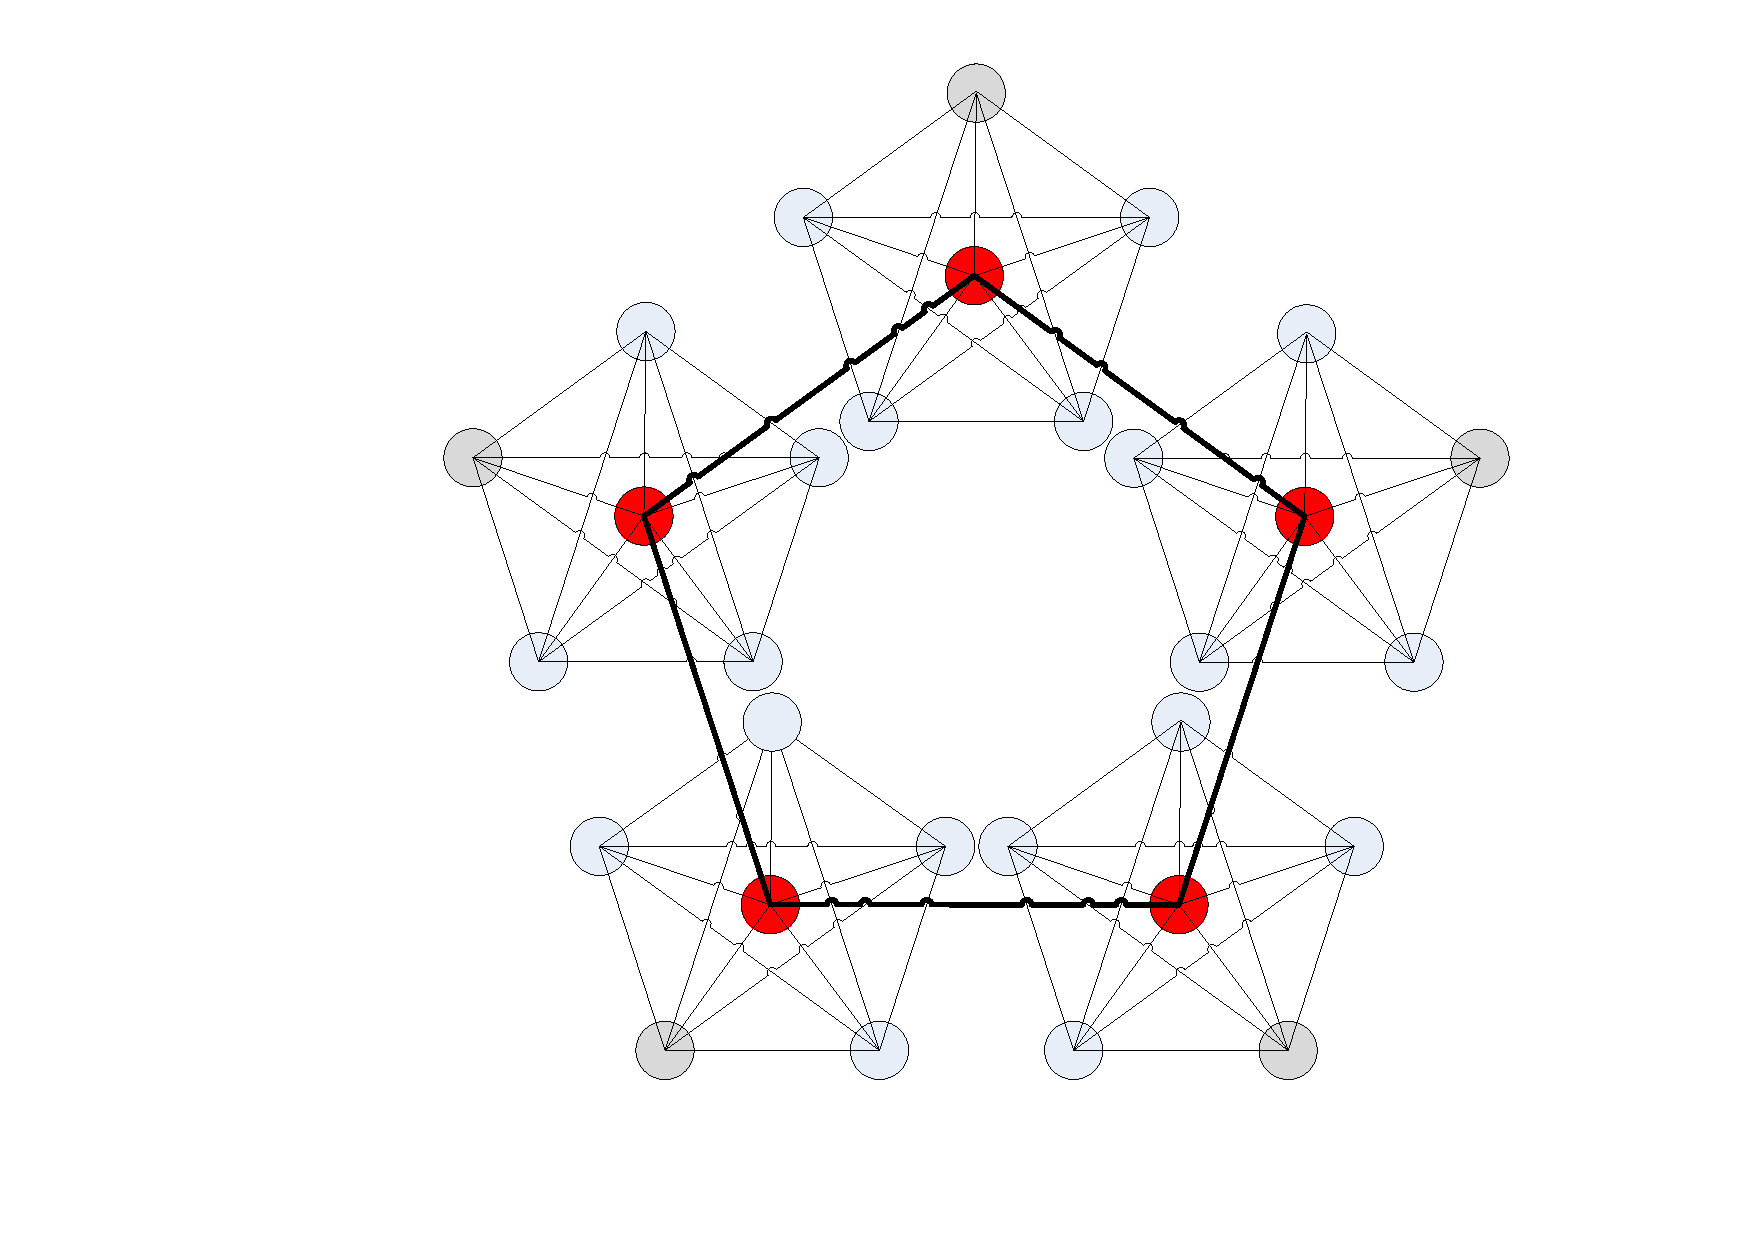
\includegraphics[clip=true, viewport=7.5cm 2.5cm 26cm 20cm, width=0.7\columnwidth]{CDHT_layout}
 \caption{Layout of the Pithos storage architecture}
 \label{fig_pithos}
\end{figure}
%
Figure \ref{fig_pithos} shows the Pithos architecture. The figure shows groups of fully connected peers (blue and red), where all groups are
connected to each other in an P2P overlay through super peers (red). This section described the general architecture of Pithos, the following
sections then describe how each of the requirements of fairness, reliability, responsiveness and security are achieved in Pithos.

Pithos groups peers in some way to form a two tiered storage model. The first tier is a storage model at group level and the second is a model over
all groups. On the first tier, which is the intra group level, a fully distributed storage system is used to allow for highly responsive read and
write operations within the group. On the second tier, which is the inter group level, overlay routing is used to store data between groups.

\subsection{Grouping}

%Speak more concretely of grouping algorithms
At the core of the architecture is how peers are grouped. Two approaches are being evaluated to group peers, one is by using distributed clustering
techniques, for example affinity propagation \cite{affinity_propagation}, the other is by using dynamic regioning techniques, for example
self-organising spatial publish subscribe (SOSPS) \cite{self_organising_sps_post}.

Distributed clustering techniques will make use of the flocking behaviour of players to dynamically group players into flocks or clusters
\cite{flocking}. The main idea of flocking is that players move around in groups, rather than randomly on their own. Because of the flocking
behaviour of players, dynamic groups or regions that move with groups of players may be a better fit than static or even dynamic regions that operate
on areas of the virtual world and not on how groups of players actually cluster. Because a fully distributed architecture is not scalable, player
density within groups should remain constant. This means that groups should merge or split as the player density in them change.

Affinity propagation clusters nodes using a similarity matrix to find similar nodes. The similarity matrix may contain any type of quantity and can
contain player positions. Affinity propagation will then group nodes depending on their location in a virtual world. This algorithm is ideally suited
to P2P applications, since it is a distributed clustering algorithm based on message passing.

As an alternative to clustering, dynamic regioning might also be used to group players. SOSPS is a new and promising development in dynamic
regioning. SOSPS creates dynamic regions based on a Voronoi overlay network \cite{voronoi_diagrams_survey}. Near constant player density is achieved
by increasing and decreasing the area sizes. This system is based on VON, a distributed Voronoi overlay network designed for MMVEs \cite{VON_VAST}.

\subsection{Store and retrieve with replication}
\label{store_retrieve}

The process of storing a file in Pithos is as follows:
\begin{enumerate}
\item A peer receives a store request from the higher game layer, along with the object that should be stored.
\item The storing peer then replicates the object $k$ times.
\item For each object, the storing peer selects a single peer from its list of group peers by sampling from a uniformly random distribution.
\item Each object is then sent to the selected peer for storage.
\item The storing peer also sends an update message to all group peers to inform them of the new object available in the group and on which peers
    the object is stored.
\item The storing peer then sends an additional replica of the object to the super peer, along with a value ($l$) specifying how many overlay
    replicas are required.
\item The group super peer generates a SHA-1 hash over the object data and uses this as the destination ID to route the overlay object to.
\item The destination super peer received the overlay object and resends it to $l$ of its overlay neighbours.
\item At each destination super peer, the super peer selects a single node in its group from a uniform random distribution where the overlay
    object is then sent to and stored.
\end{enumerate}

Currently, Pithos sends the object along with a store request to the group super peer, where the group super peer then forwards that object to
another super peer and that super peer then sends the object to a group peer for storage. A future improvement might be to only send signalling
messages to the nodes in the forwarding path that indicate that a source node has an object to store. When the signalling message then arrives at the
different destination nodes, they can contact the source node directly and obtain the object from that node. This will reduce the amount of bandwidth
consumed by the storage operation.

The process of retrieving a file from Pithos is as follows:
\begin{enumerate}
\item A peer receives a retrieve request from the higher game layer that contains the object ID generated from the SHA-1 hash.
\item The peer then searches for the object in its list of group objects.
\item If the object is available in the group, the object is requested from the peer containing it and sent up to the game layer.
\item If the object is not available in the group, an object request is sent to the group super peer.
\item The group super peer requests the object by ID, forwards the received object to the requesting peer where the requesting peer then sends
    the object to the game layer.
\end{enumerate}

Pithos implements data replication to enable it to handle node churn. If a node leaves the network and stops to transmit pong messages, the migration
mechanism will detect this and replicate the file on another node. Replication exists intra as well as inter group.

\subsection{Secure storage and node ID assignments}
\label{secure_ids}

In order to design a secure distributed storage system, one requirement for the P2P overlay is that nodes should not be able to select their own IDs
or it will not be possible to secure the system against attack. Node IDs should rather be assigned securely by some certification authority
\cite{secure_overlay_routing}.

To this end Pithos implements its own certification authority to assign node IDs securely and promote security in the P2P overlay. A certification
server exists that handle ID requests from nodes. The server assigns IDs to nodes and provides the node with a signed certificate that it may use to
store data.

Whenever objects are stored or updated in the storage network, nodes have to sign the object with their certificate to enable the tracking of object
changes throughout the life of the object. This system is very different from classic distributed file storage designs that advocate anonymity in
storage. The fact that all changes can be tracked to a specific node will simplify the task of eliminating player cheating.

Other security safeguards exist that have to be implemented in the P2P overlay in order to create a secure system. Secure node ID assignments are
mentioned here, since this cannot be implemented in the overlay used, but has to be implemented in the higher layer application (Pithos) making use
of a P2P overlay (Pastry, Chord, Kademlia).

\subsection{Distance-based storage} \label{distance_based}

For Pithos to perform well as an MMVE storage architecture, intra-group data requests should be preferred to inter-group data requests. This
requirement, combined with the fact that the grouping algorithm geographically groups players, lends Pithos to a storage system based on
distance-based storage. The assumption made is much the same as the one made for interest management, that players have a limit area of interest and
require interaction with a limited number of objects within range.

The design is then to implement distance-based storage, but on a group level rather than an individual level. This means that objects are stored on
the nearest group of players, rather than the nearest player. It is supposed that such an approach will also alleviate many of the challenges present
with distance-based storage as discussed in the following subsections.

With group-based distance-based storage, it is assumed that because peers now store objects closest to the group, the objects that they are
interested in will most likely be stored within their own group. What follows is that most data requests should be intra-group requests. The overlay
storage component ensures that nodes that require data not stored within their group are still able to access the data.

\section{Pithos evaluation}

This section evaluates the Pithos design according to the requirements set out in Section \ref{current_models} of responsiveness, reliability,
fairness, security and scalability.

\subsection{Responsiveness}

Responsiveness is achieved by allowing players to store data within their group and presenting them with direct access to data anywhere in the group.
It is assumed that player requests will be for data that are mostly contained within their groups, thereby prioritising the faster intra group
communications as opposed to the slower overlay communications. It should be noted that because group storage is faster than overlay storage, any
percentage of intra-group messages will improve the responsiveness of the system beyond that of overlay storage.

If players are grouped intelligently and group migration does not occur often, less traffic will have to flow between groups, which will reduce the
number of queries to the DHT, which in turn will improve the latency of the overall system.

Some preliminary results on the responsiveness of Pithos is presented in Section \ref{responsiveness_results}.

\subsection{Fairness}

Two areas of fairness are explored in the Pithos storage system. The one is group object fairness and the other is overlay object fairness. Group
objects are stored by peers storing objects within their own group, overlay objects are stored by the super peer in the overlay. From the storage
description of Section \ref{store_retrieve}, it is evident that overlay objects are also stored amongst all nodes in the network and that peers
contain a mixture of overlay and group objects.

To evaluate the fairness, we evaluate the standard deviation of the number of objects stored per peer. To make the storage of group objects fair,
every node in a group can by picked at a probability sampled from a integer uniform distribution, where the maximum value of the distribution is the
number of nodes in the group. This selection mechanism produces objects distributed normally around some average as can be seen from the preliminary
results presented in Section \ref{fairness_results}.

The mapping of overlay objects to nodes are done differently. Because P2P overlays use distance-based routing, objects are stored on the node with an
ID that is closest to the ID of the file stored. This storage method in effect maps objects to nodes, where every node covers a different area of the
key space. The distribution of objects for this type of storage is less fair than group storage, with a higher standard deviation and longer tail.

It should however be noted that distribution of overlay objects are just as fair as for any overlay storage technique and much fairer than a super
peer storage technique. Some preliminary results on the fairness of overlay storage is also presented in Section \ref{fairness_results}.

\subsection{Reliability}

The Pithos replication and migration mechanisms should ensure reliable storage. Objects are replicated and can be migrated to new nodes if a player
has left the network. As long as files can be migrated faster than what it would take for all replicas to leave the network, the system will remain
reliable. One also doesn't expect high levels of churn in an MMVE, with typical sessions lasting for one or two hours before a user leaves the world.

The group-based distance-based architecture of Pithos also improves reliability in that data are now more resistant to churn because grouping allows
for migration. This method provides a concrete method by which distance-based storage can be made reliable, something that has not been found in the
literature.

\subsection{Security}

It is believed that the secure node ID assignments and storage certification described in Section \ref{secure_ids} greatly improves the security of
Pithos over other architectures that have thus far been presented. In fact, very little storage architectures address the security issues present in
state persistency for P2P MMVEs.

Another advantage of the group-based distance-based storage presented here is that the security issue mentioned in Section
\ref{classic_distance_based} is much less of a concern. Because data are now stored on the nearest groups and not the nearest players, it makes it
much more difficult to cheat. This is achieved by the group replication mechanism as well as the possibility to add hash checking to the retrieval
process. An object can now be retrieved from one group peer and hashes can be requested from other group peers. The hashes can be compared to a hash
of the file received, which would enable a requesting node to determine whether a file has been altered.

Also, because all file updates must be signed by a certificate and every node is uniquely identified by its certificate, the malicious node can be
tracked and dealt with.

\subsection{Scalability}

The protocols used in Pithos have been designed with scalability in mind. The issue of group sizes becoming to large have been addressed and ways
have been proposed by which player density in groups can be kept constant. This will ensure that traffic in groups remain constant. The other
component used is the P2P overlay, which is by design scalable.

That said, the amount of network traffic present should still be measured, this can however only be done after the amount and characteristics of the
storage traffic is known for an MMVE.

\subsection{Future work}

The issue with such a system would be how to uniquely identify a group and how the identification would be applied when groups merge or split. Groups
moving towards each other also have to be identified and the grouping might have to be able to maintain two groups moving through each other. Little
work has been done to group players in a distributed fashion in virtual worlds. Further research is required into grouping algorithms to determine
their usability in virtual worlds under user churn.

The simulation does not yet support nodes leaving the network. The migration mechanism should still be implemented before rigourous testing under
heavy network churn will become a possibility.

%Don't send complete files

%Use KBRTestApp

\section{Preliminary results}
\label{results}

Pithos is currently still a work in progress, but for preliminary results the requirements of responsiveness and fairness were measured.
Responsiveness is defined as how long it takes to store and retrieve a node from the network. Fairness is defined as the standard deviation in the
number of files or bytes stored on the different nodes.

The responsiveness is compared to Pastry routing times.

\subsection{Test setup}

Pithos is being implemented in Oversim \cite{OverSim_2007}, running on Omnet++. Oversim was chosen because of the variety of already implemented
protocols as well as the layered architecture, which simplifies testing with different overlays and comparing with different storage types.

In the results shown, Pastry was used as the P2P overlay and Pithos was driven by a \emph{game} module. After a node has joined a group, the game
module starts to generate store and retrieve requests. Pastry was chosen because of many articles referencing Pastry as the overlay used for overlay
storage. It should be noted that because of Oversim's layered architecture, Pithos can work and has been additionally tested with the Chord and
Kademlia overlays. The ideal choice of overlay is a question for future research and testing.

For the results shown in Section \ref{results}, 14999 peers, 499 super peers and a single directory server are created at the start of the
simulation. The directory server publishes super peer information, which allows a peer to join the group nearest to it. Because of the way Pithos is
structured, each super peer node is also a peer node, which then gives a total of 15000 Oversim nodes. This limit is established by the number of
node coordinates in the Oversim coordinates file, but can later be expanded when a larger coordinates file is found.

After a specific node has joined a group, it informs the game module and the game module then starts to generate store and retrieve requests. These
requests are received by Pithos and handled. Pithos was configured to store two group replicas and one overlay replica for every root object stored
to give a ratio of group storage to overlay storage of 3:1.

\subsection{Responsiveness}
\label{responsiveness_results}

Firstly, we evaluate the responsiveness of the storage system. In the storage system, we expect two levels of responsiveness. We expect a certain
level of responsiveness for intra group communications and a certain level of responsiveness for inter group communications.

We can calculate an average response time which is determined by the percentage of intra group requests, compared to inter group requests as follows:
%
\begin{equation}\label{expected_response_time}
    E[T_{\textrm{resp}}] = \left(P(g)\left(E\left[T_{\textrm{group}}\right]\right) + \left(1 - P(g)\right)\left(E\left[T_{\textrm{overlay}}\right]\right)\right)
\end{equation}
%
, where $E[T_{\textrm{resp}}]$, the expected value of the overall system response time is given by $P(g)$, the probability that a message is routed
within a group, $E\left[T_{\textrm{group}}\right]$, the expected value of the root and replica message distribution as shown in Figure
\ref{fig_pithos_response} and $E\left[T_{\textrm{overlay}}\right]$, the expected value of the overly message distribution also shown in Figure
\ref{fig_pithos_response}.

\begin{figure}[htbp]
 \centering
 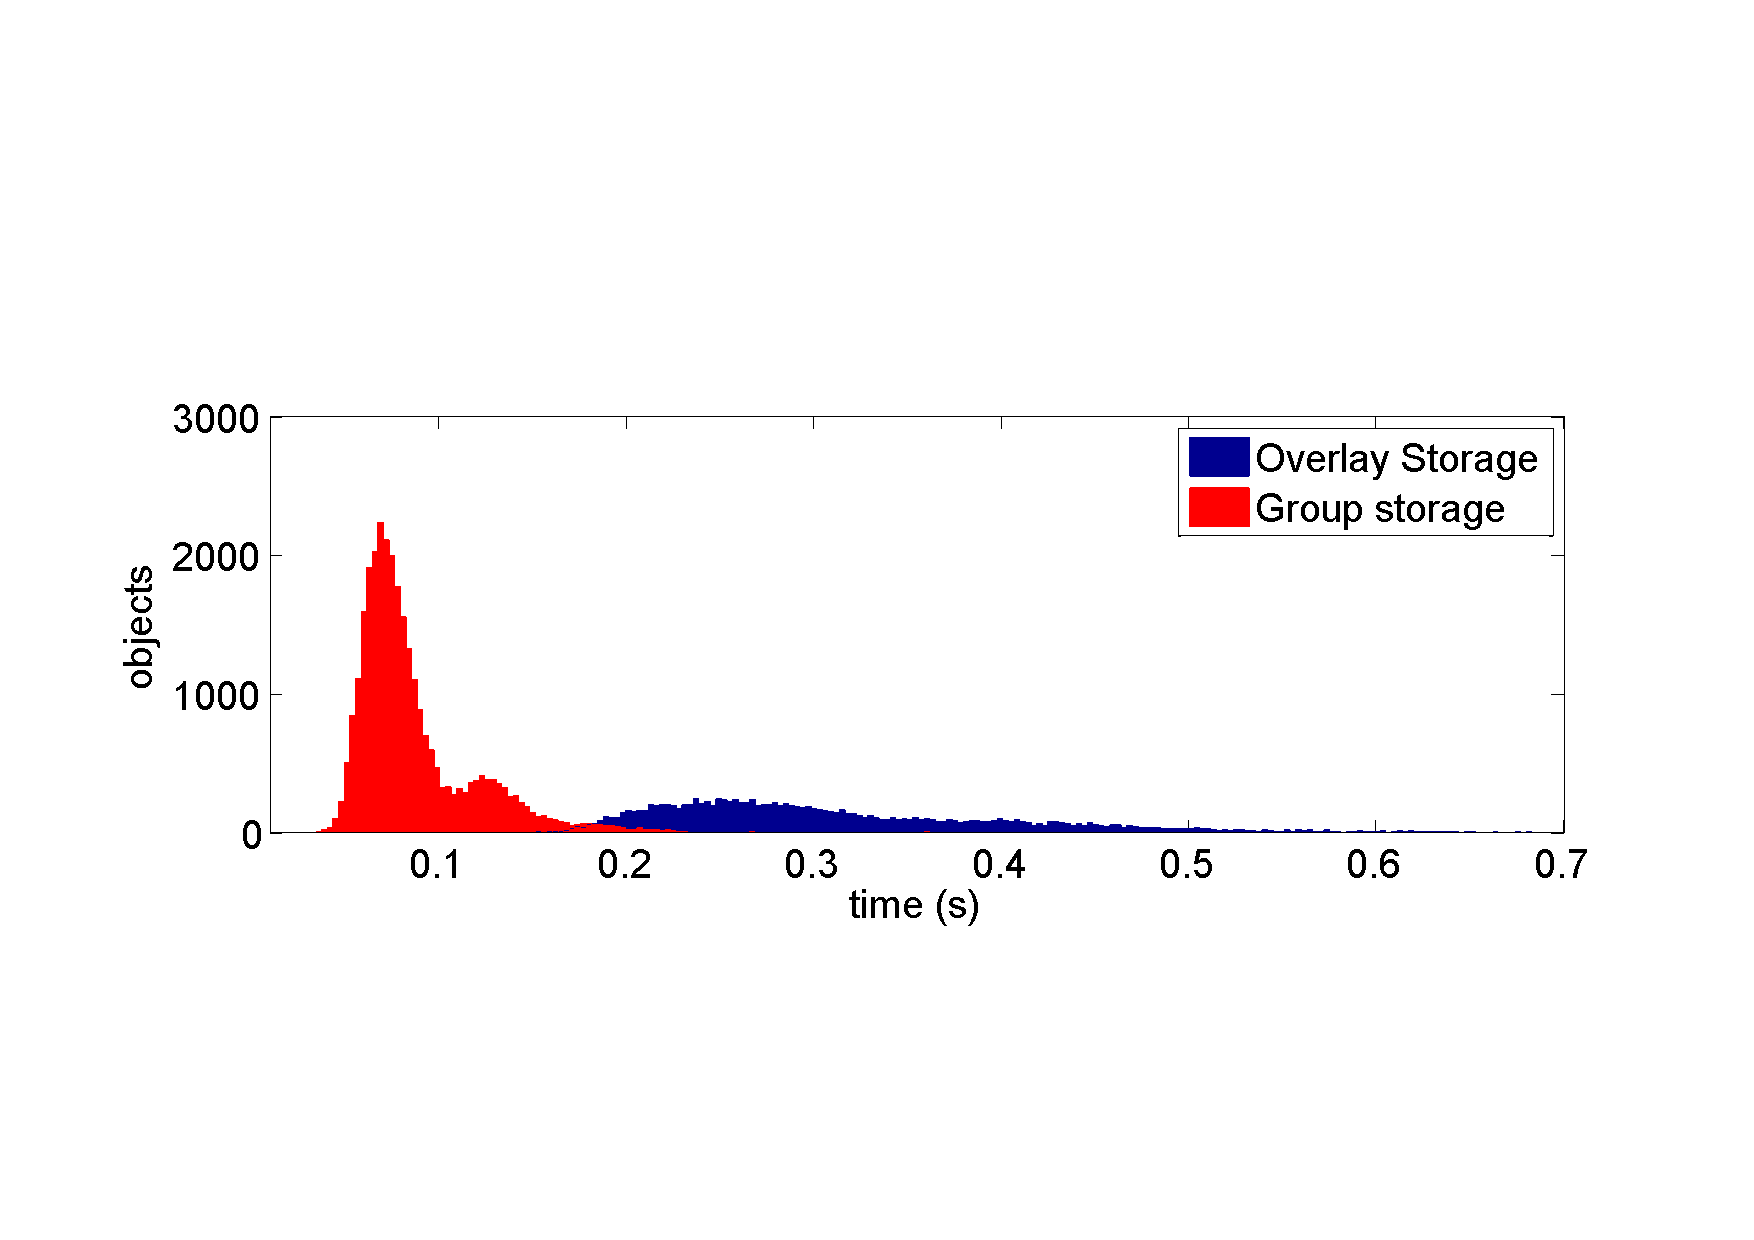
\includegraphics[clip=true, viewport=1.5cm 1.3cm 25.5cm 19.7cm, width=\columnwidth]{request_time_distribution}
 \caption{Time distribution of overlay and root/replica objects}
 \label{fig_pithos_response}
\end{figure}
%
Figure \ref{fig_pithos_response} shows the distribution of mean storage request times over all nodes in the network for the different types of
storage present in the network. One can see that the intra group root and replica objects are stored much faster than the overlay objects in the
network. Specifically, intra group object are stored with an expected time of $E\left[T_{\textrm{group}}\right] =  0.0878 s$, while inter group
objects are stored with an expected time of $E\left[T_{\textrm{overlay}}\right] = 0.3284 s$, 3.74 times slower than intra group storage.

There seem to be multiple distributions of root and replica nodes spaced equally apart. The supposition is that these represent the physical hops in
the underlaying architecture.

From Figure \ref{fig_pithos_response} it is evident that if only overlay storage is used, the storage and retrieval times will be much higher. To
exactly compare Pithos with overlay storage, the percentage of intra group requests ($P(g)$) should first be known. At this time there is no way to
know what this percentage is, but the responsiveness can be calculated as a function of $P(g)$. From Equation \eqref{expected_response_time}, if
there are no intra-group messages in the system ($P(g) = 0$), the system performs as well as overlay storage. For any $P(g) > 0$, the system performs
better than overlay storage.

The responsiveness of Pithos will of course depend on the number of nodes in the network ($N$). This is because the number of routing hops in a P2P
overlay is dependant on $N$, specifically for Pastry \cite{storage_and_chaching_PAST}:
%
\begin{equation}\label{pastry_hops}
    E[H_{\textrm{pastry}}] = \log_{2^b}\left(N\right)
\end{equation}
%
, where $E[H_{\textrm{pastry}}]$ is the expected number of Pastry hops and $b$ is a network parameter that is usually chosen $b = 4$. From this, it
is possible to calculate a theoretical performance for Pithos and compare that with a theoretical performance of overlay storage.

As with Equation \eqref{expected_response_time}, a weighted hop average will be used to calculate expected hops for both Pithos and overlay storage
for various numbers of nodes as follows:
%
\begin{equation}\label{expected_response_time}
    E[H] = P(g)\left(E\left[H_{\textrm{group}}\right]\right) + \left(1 - P(g)\right)\left(E\left[H_{\textrm{overlay}}\right]\right)
\end{equation}
%
, where $E[H]$ is the expected number of Pithos hops, $E\left[H_{\textrm{group}}\right]$ is the expected number of group hops and
$E\left[H_{\textrm{overlay}}\right]$ is the expected number of overly hops. In Pithos, the expected number of group hops is
$E\left[H_{\textrm{group}}\right] = 1$, because in a fully connected group any node is always one hop away from any other node.

To find the value of $E\left[H_{\textrm{overlay}}\right]$, one has to look at how many hops an overlay messages required in Pithos. A message store
request is generated on a group peer. That group peer forwards the message to its group super peer, which is always a single hop away. The super peer
then forwards the message to another super peer in $\log_{16}(M)$ hops, from Equation \eqref{pastry_hops}, where $M$ is the number of super peers in
the network. From the destination super peer, another hop is required to send the message to the destination group peer. This gives
%
\begin{equation}\label{group_hops}
    E\left[H_{\textrm{group}}\right] = 1 + \log_{16}(M) + 1.
\end{equation}
%
Equation \eqref{expected_response_time} then becomes:
%
\begin{equation}\label{expected_response_time_exp}
    E[H] = P(g) + \left(1 - P(g)\right)\left(2 + \log_{16}\left(M\right)\right).
\end{equation}

\begin{figure}[htbp]
 \centering
 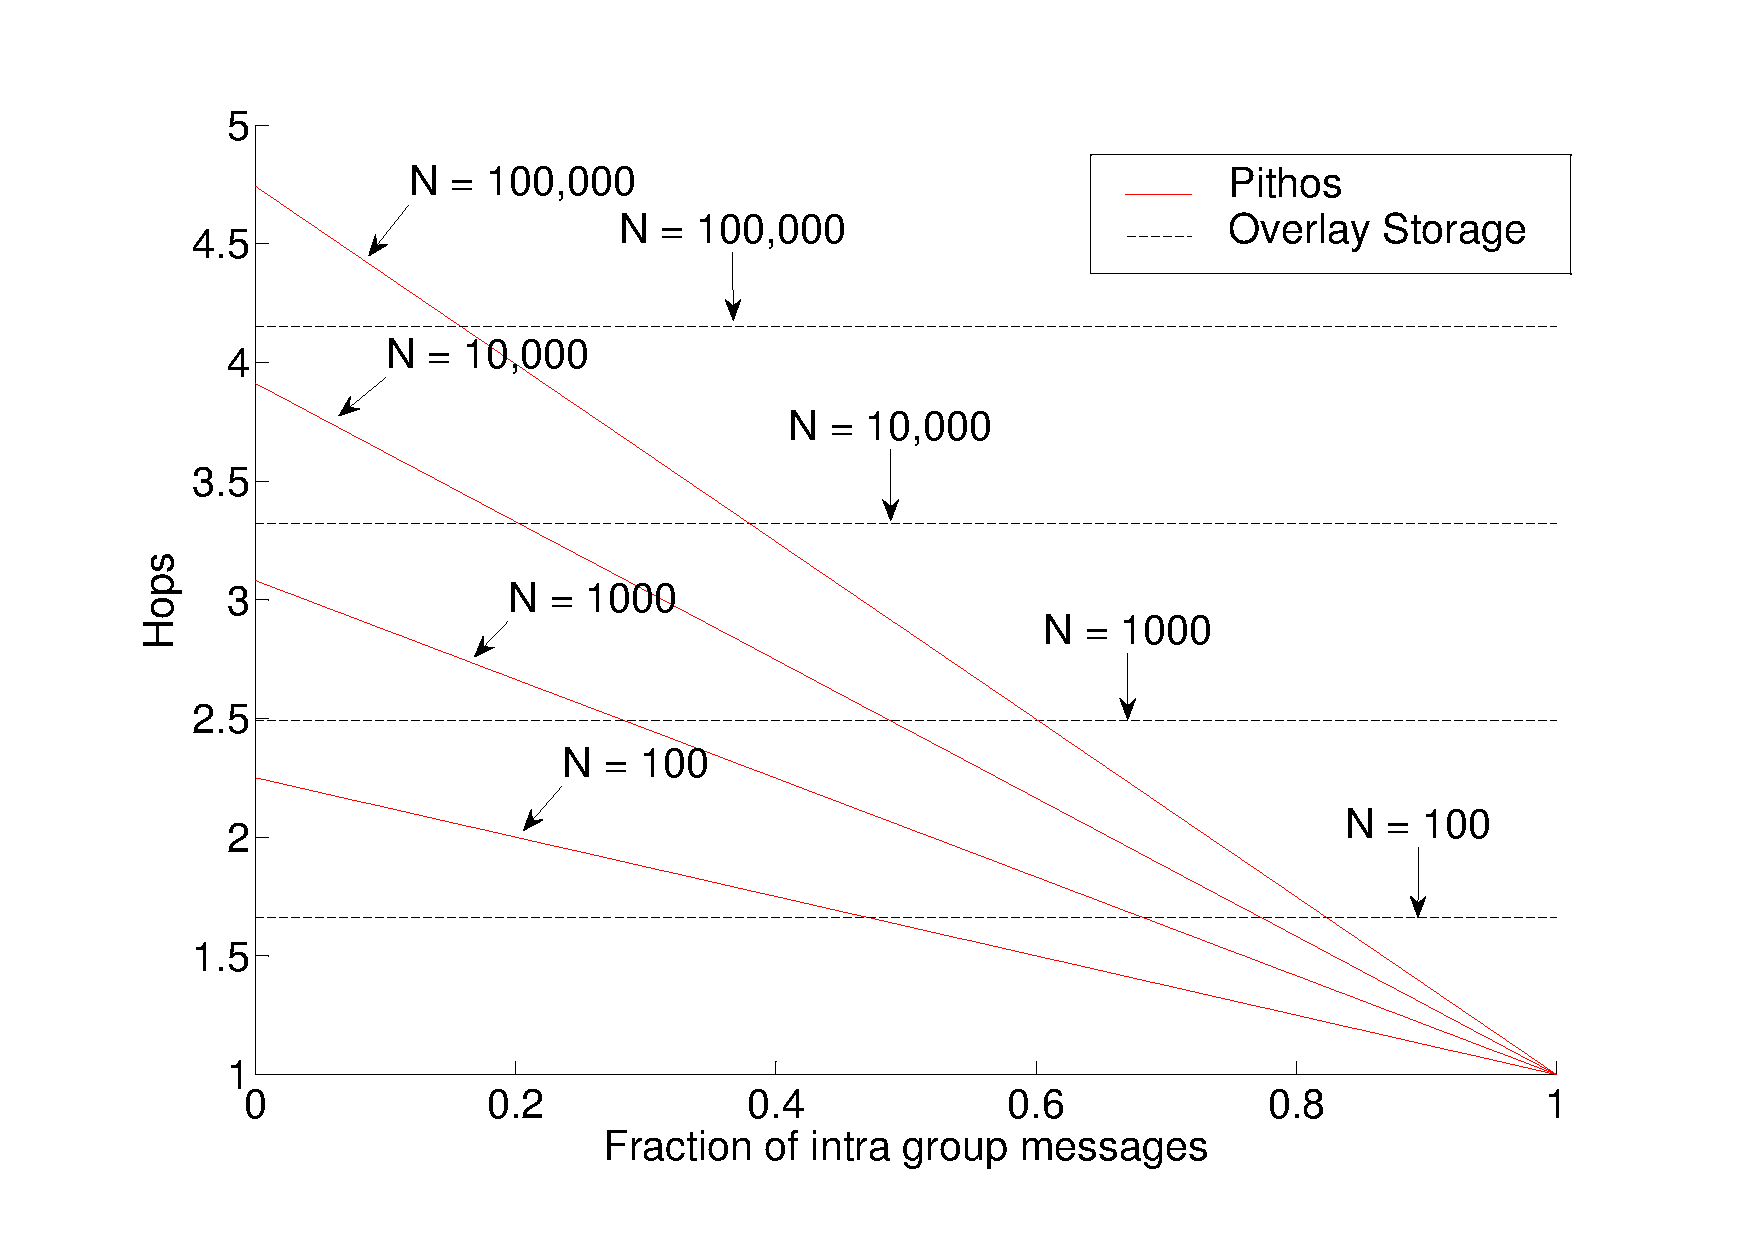
\includegraphics[clip=true, viewport=2cm 1cm 27cm 19.5cm, width=\columnwidth]{Hops_vsGroupFrac_4n}
 \caption{Time distribution of overlay and root/replica objects}
 \label{fig_hop_compare}
\end{figure}
%
Figure \ref{fig_hop_compare} compares the expected number of Pithos hops with the expected number of overlay hops as a function of intra-group
probability ($P(g)$) for numbers of nodes ($N$). The overlay hops were calculated from Equation \eqref{pastry_hops}, while the Pithos hops were
calculated from Equation \eqref{expected_response_time_exp}. For the Pithos graphs, an average number of 50 peers per group was used to determine the
number of super peers.

Figure \ref{fig_hop_compare} shows that for a low value of $P(g)$, overlay storage performs better than Pithos because of the additional two hops
present in Pithos. For 10,000 nodes Pithos starts to perform better then overlay storage when $P(g) > 0.2$. This is considered a low value for
$P(g)$, because of the distance-based design of Pithos that attempts to maximise the value for $P(g)$. It should be noted that Pithos also seems more
scalable than overlay storage, since the threshold value for $P(g)$ becomes lesser, the more nodes there are in the network.

\subsection{Fairness}
\label{fairness_results}

\begin{figure}[htbp]
 \centering
 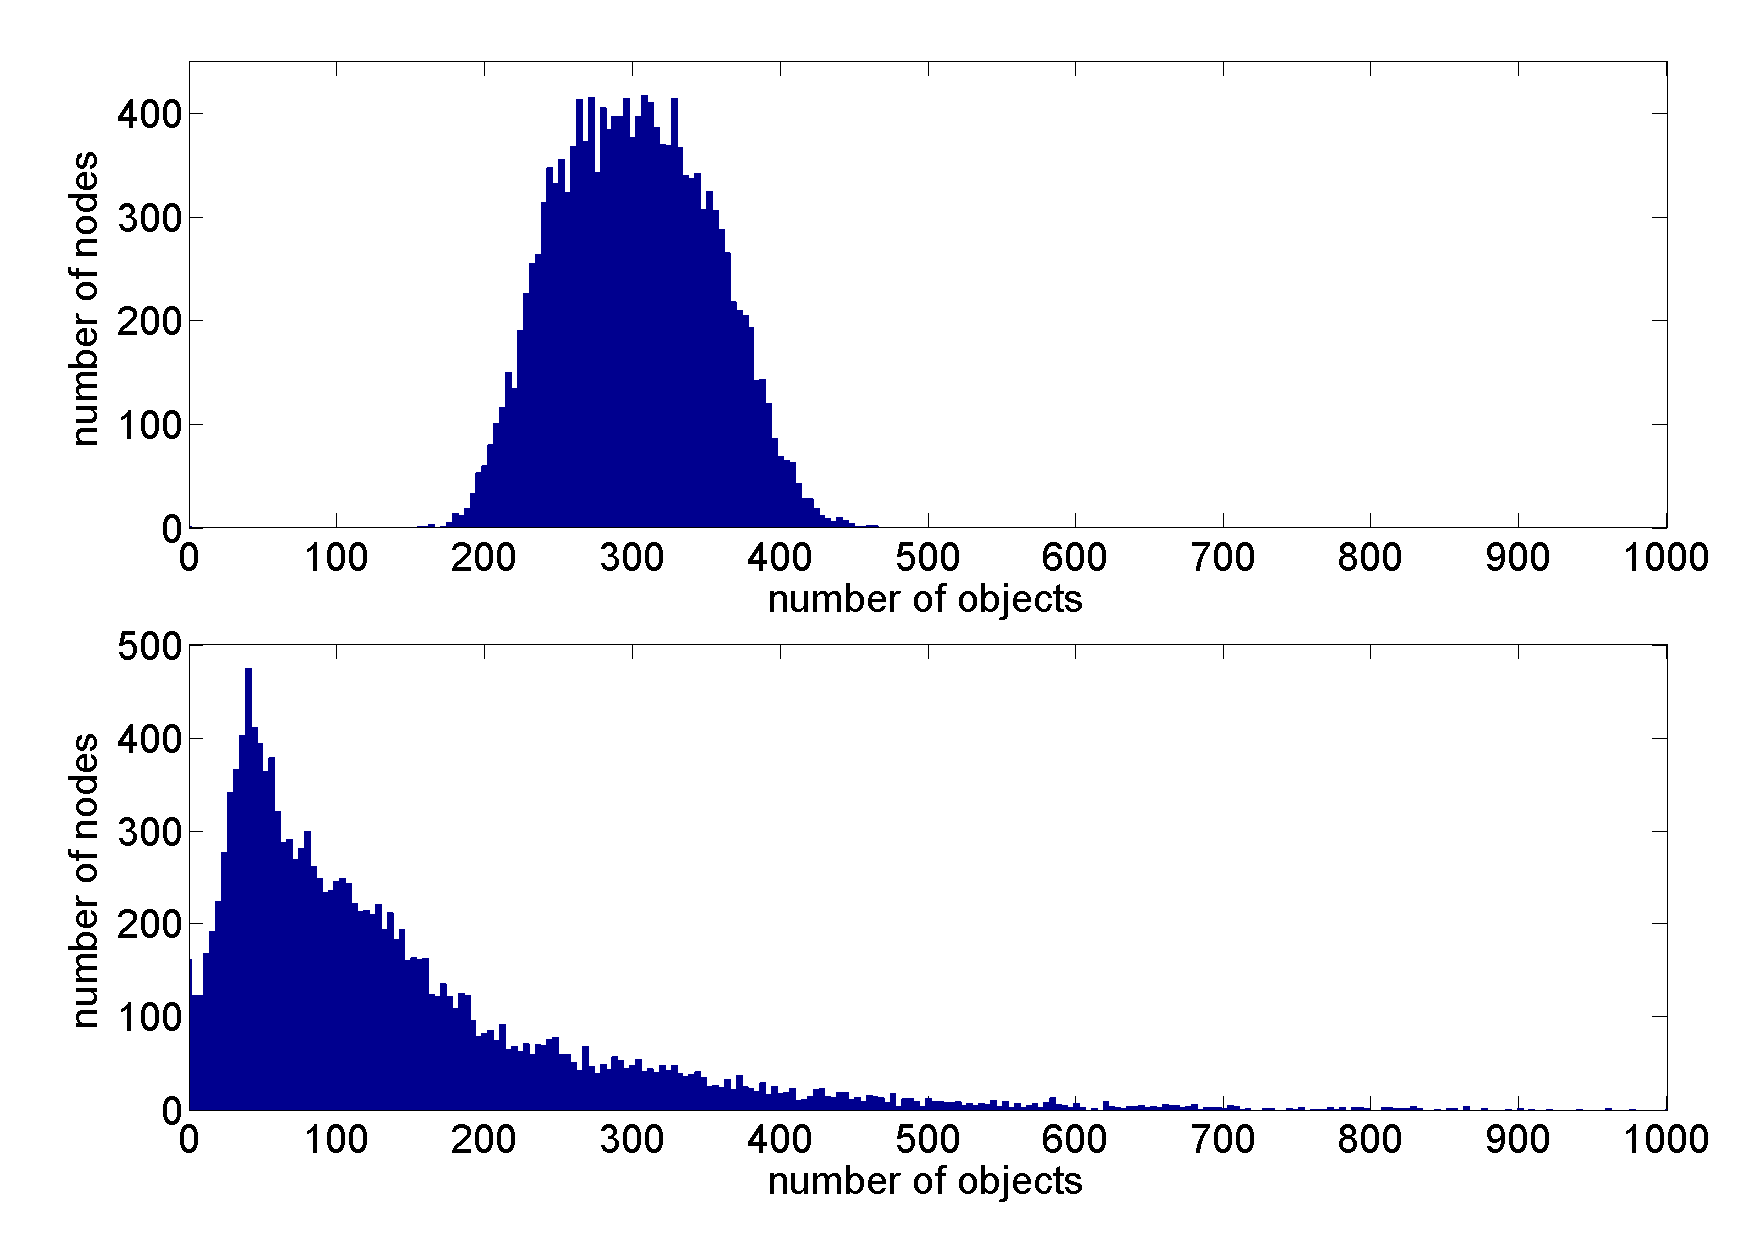
\includegraphics[clip=true, viewport=1cm 0.5cm 28.5cm 20cm, width=\columnwidth]{RootRepOverlayObjects}
 \caption{Root/Replica object number distribution}
 \label{fig_group_overlay_objects}
\end{figure}
%
%\begin{figure}[htbp]
% \centering
% 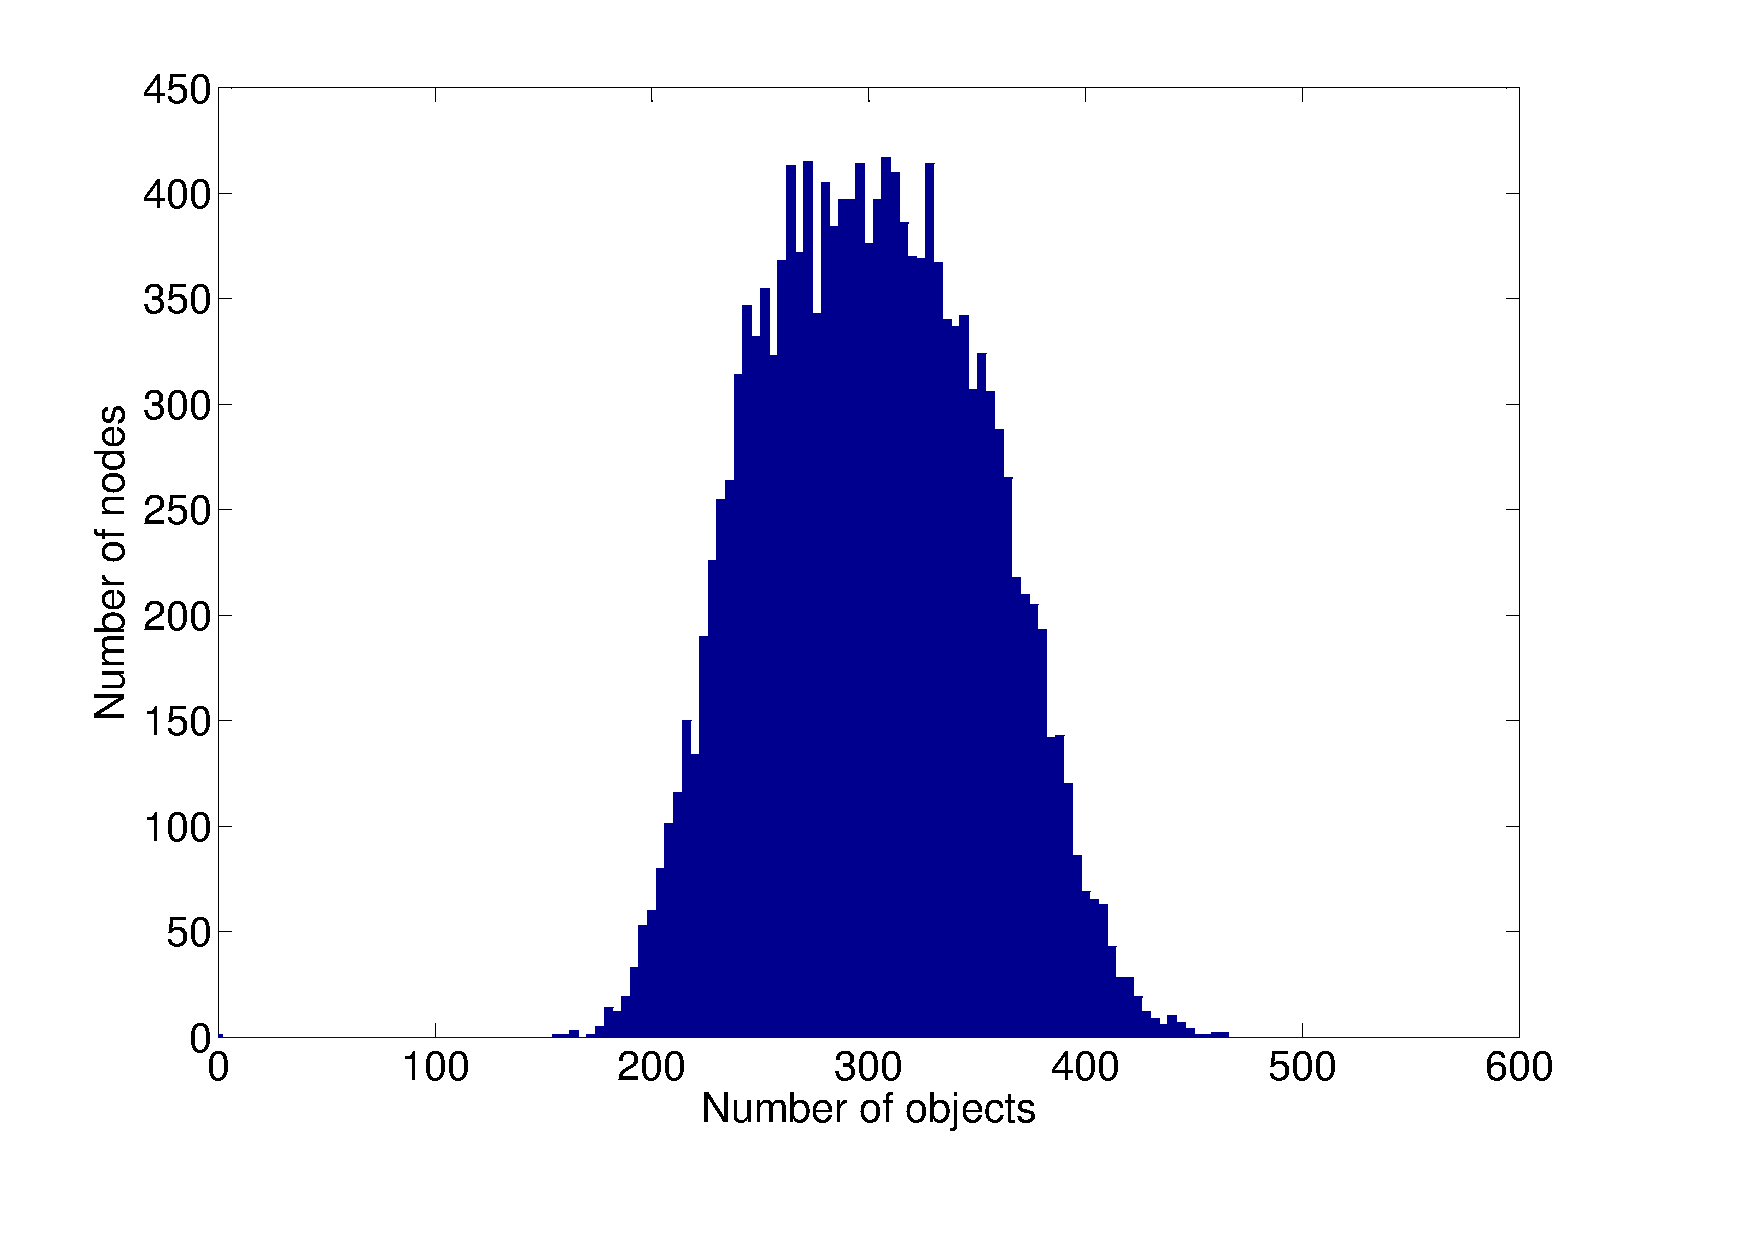
\includegraphics[clip=true, viewport=1.5cm 1.8cm 26.5cm 20cm, width=\columnwidth]{RootRepObjects}
% \caption{Root/Replica object number distribution}
% \label{fig_group_objects}
%\end{figure}
%
To measure fairness, the object distributions over the nodes in the network are investigated. Figure \ref{fig_group_overlay_objects} (top) shows the
distribution of group objects over nodes in the network. The figure shows how many nodes store how many objects. From this figure it is evident that
the object distribution forms a normal distribution. The distribution has a mean of 302 objects per node and a standard deviation of 51 objects per
node.

%\begin{figure}[htbp]
% \centering
% 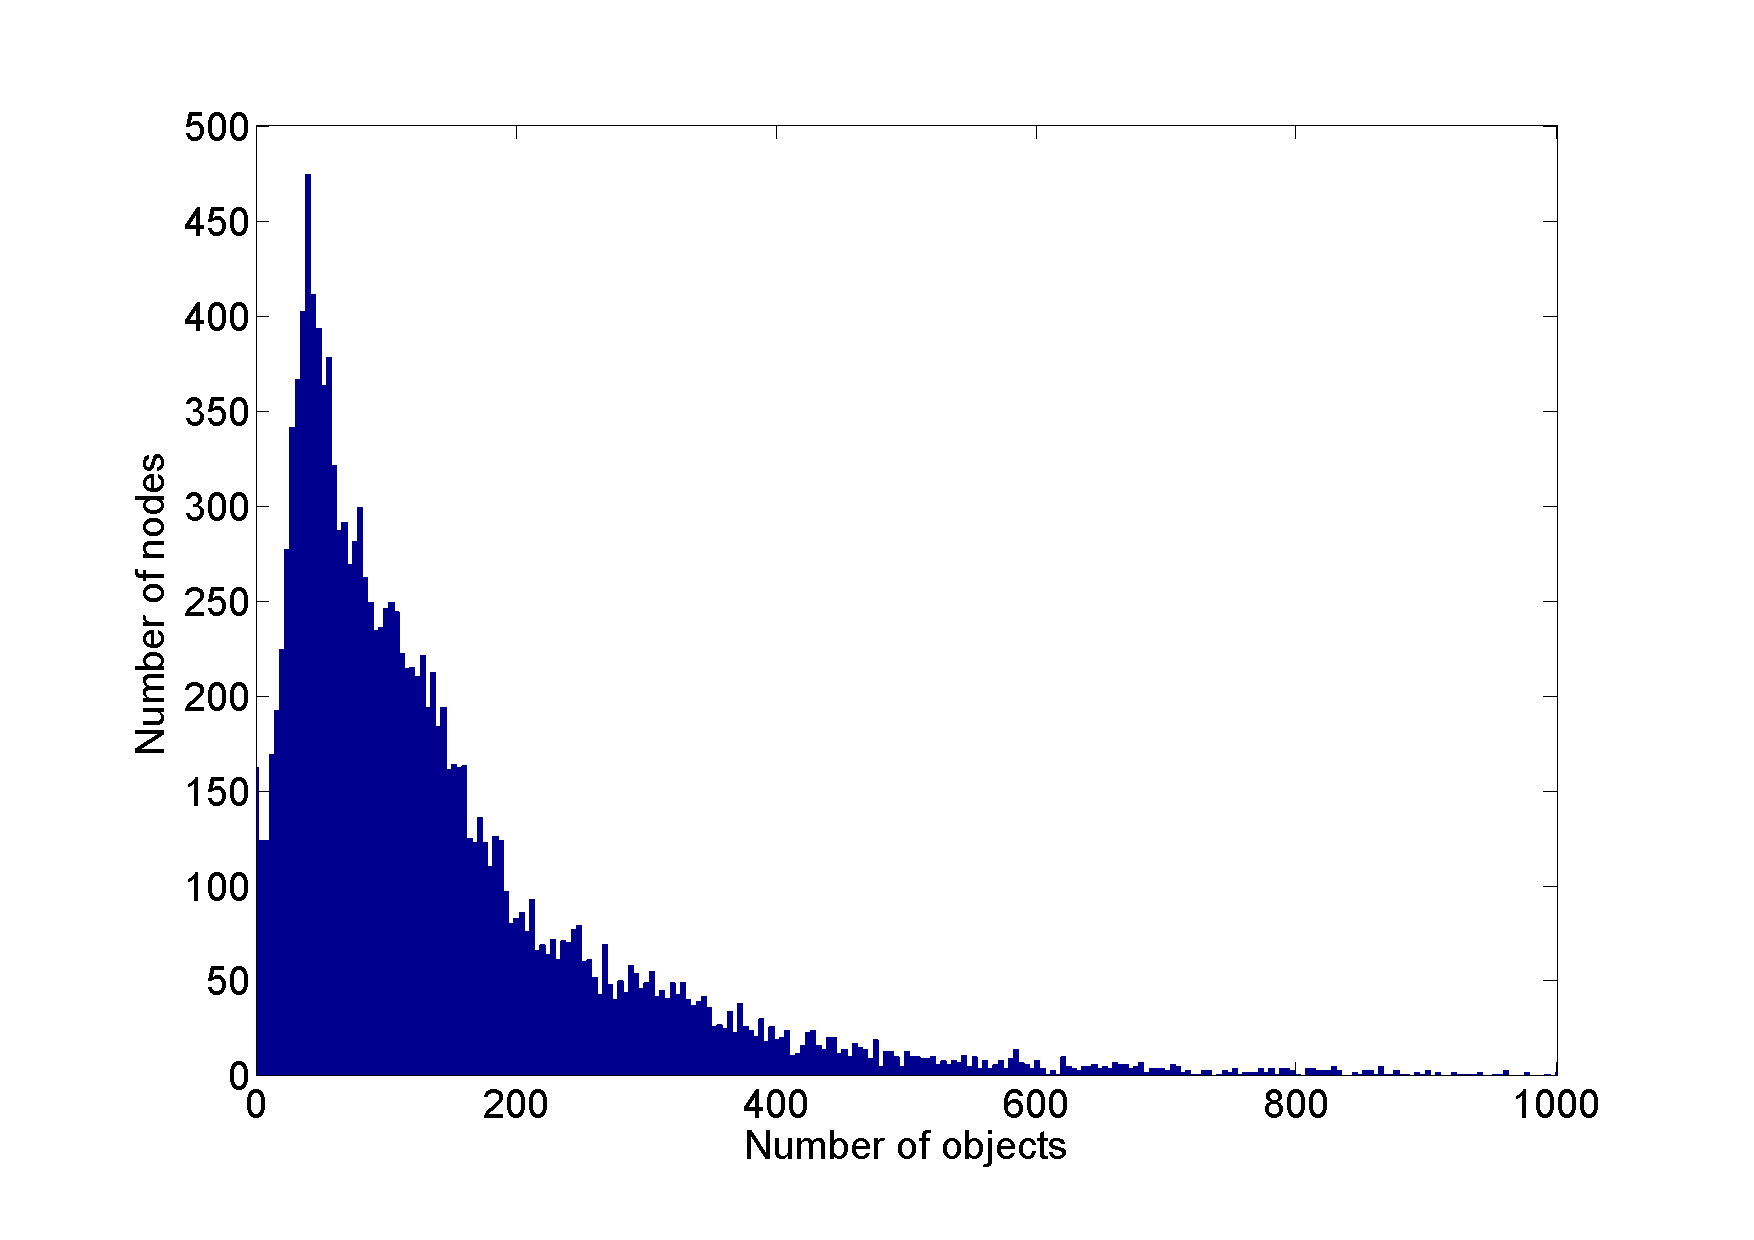
\includegraphics[clip=true, viewport=1.5cm 1.2cm 27cm 19.7cm, width=\columnwidth]{OverlayObjects}
% \caption{Overlay object number distribution}
% \label{fig_overlay_objects}
%\end{figure}
%
Figure \ref{fig_group_overlay_objects} (bottom) shows the distribution of overlay objects in Pithos. The distribution has a mean of 153 objects per
node and a standard deviation of 189 objects per node. Comparing group storage to overlay storage, it is also evident that group storage is much
fairer than overlay storage, if the standard deviation is taken as a measure of fairness. This shows that designing a hybrid system which prefers
group storage to overlay storage, one is also designing a fairer system than overlay storage. It should be again noted here that super peer storage
is not being considered, because of its complete lack of fairness.

The reason why overlay storage is not particularly fair is not at first evident. At first glance, one might think that mapping one uniform
distribution (the file ID hashes) to another uniform distribution (the node ID hashes) in a distance-based manner would produce a system where the
number of files per node is roughly balanced \cite{storage_and_chaching_PAST}. This is not the case. The key is that uniformly distributed does not
mean evenly distributed. In other words, if numbers are sampled from a uniform random distribution, the differences between consecutive numbers will
not be at all similar. This shows that although overlay storage distributed files over all nodes, the number of files per node can vary greatly.

\begin{figure}[htbp]
 \centering
 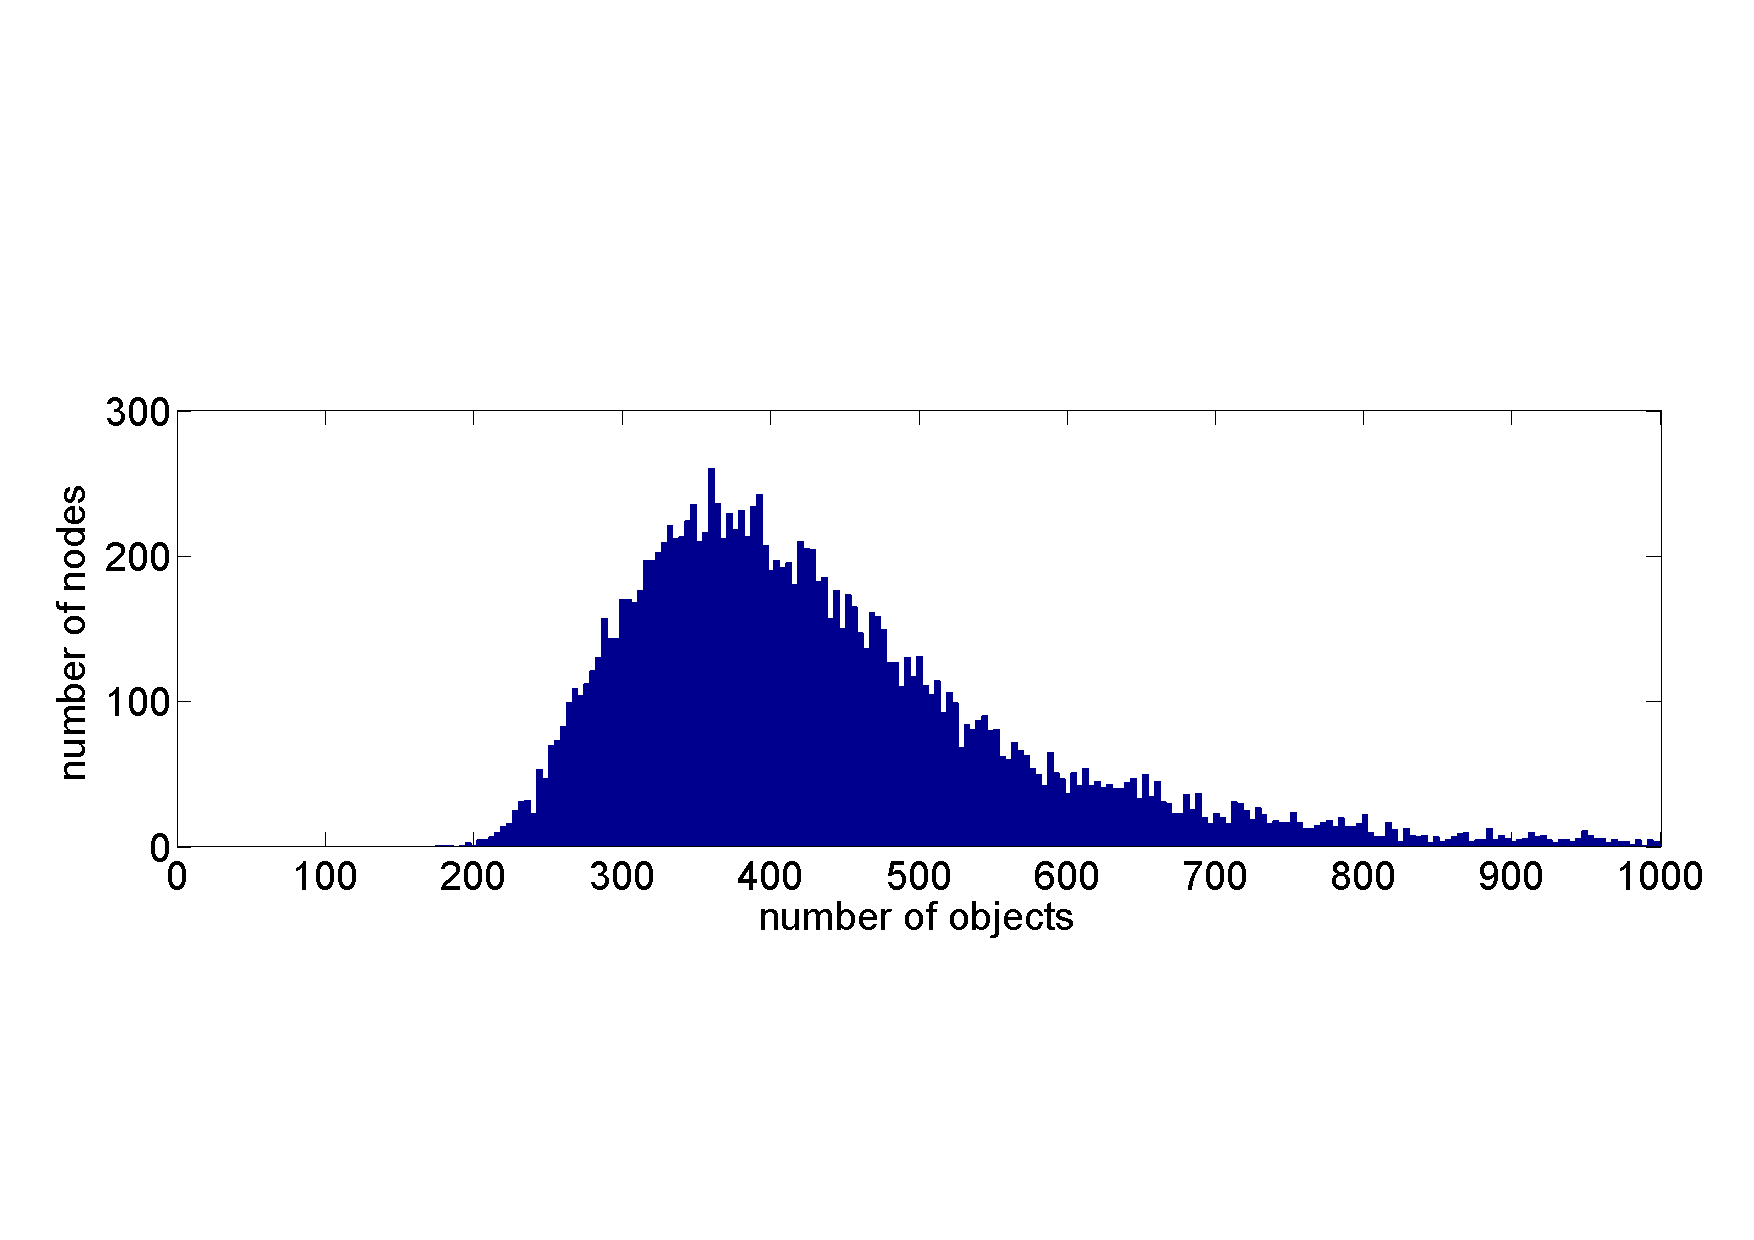
\includegraphics[clip=true, viewport=1cm 5cm 29cm 14.5cm, width=\columnwidth]{Objects}
 \caption{Combined object number distribution}
 \label{fig_objects}
\end{figure}
%
Figure \ref{fig_objects} shows the combined object distribution of Pithos. The distribution has a mean of 453 objects per node and a standard
deviation of 200 objects per node or 44\%. The overall fairness of Pithos is thus significantly better than the fairness of overlay storage.

%\begin{figure}[htbp]
% \centering
% 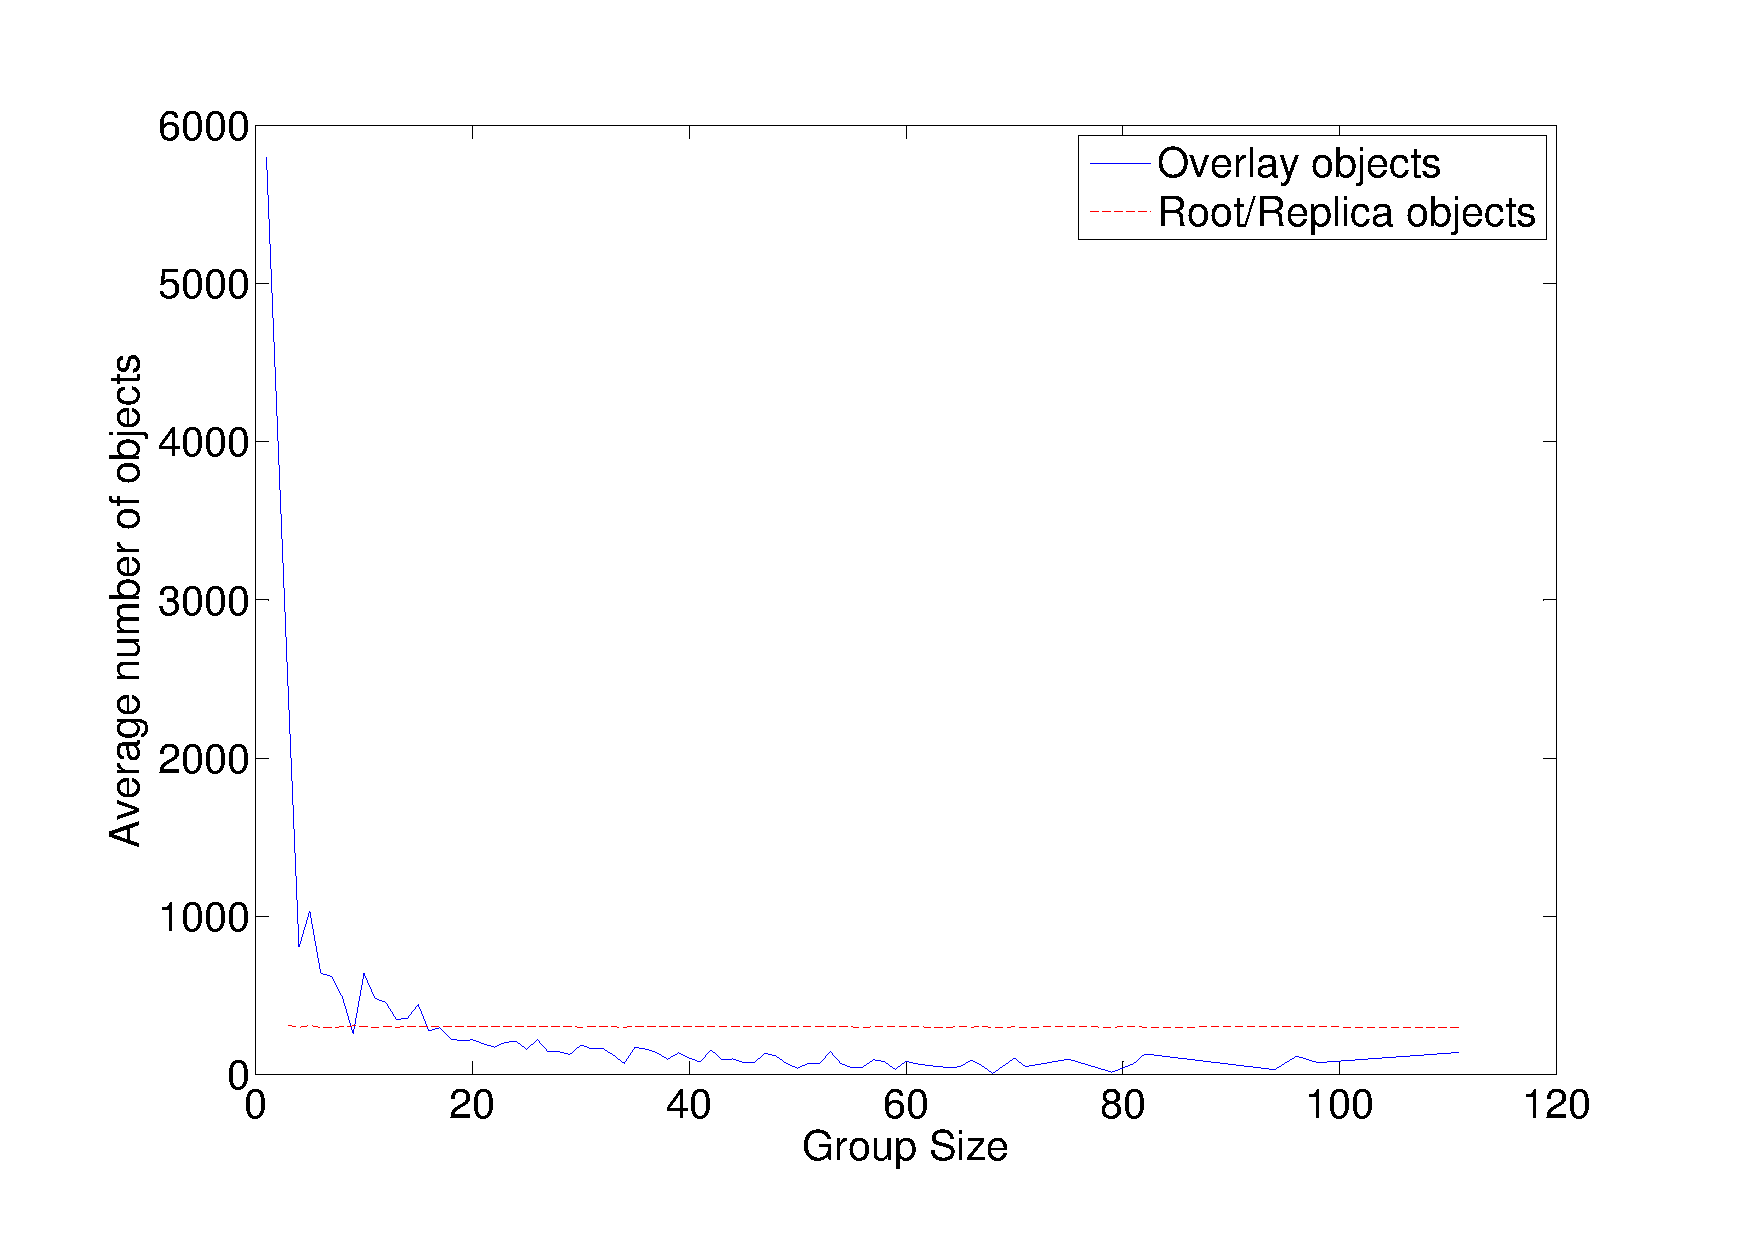
\includegraphics[clip=true, viewport=1.5cm 1cm 27cm 19.5cm, width=\columnwidth]{ObjectsByGroupSize}
% \caption{Average number of overlay objects stored by group size}
% \label{fig_objects_by_groupsize}
%\end{figure}
%
\begin{figure}[htbp]
 \centering
 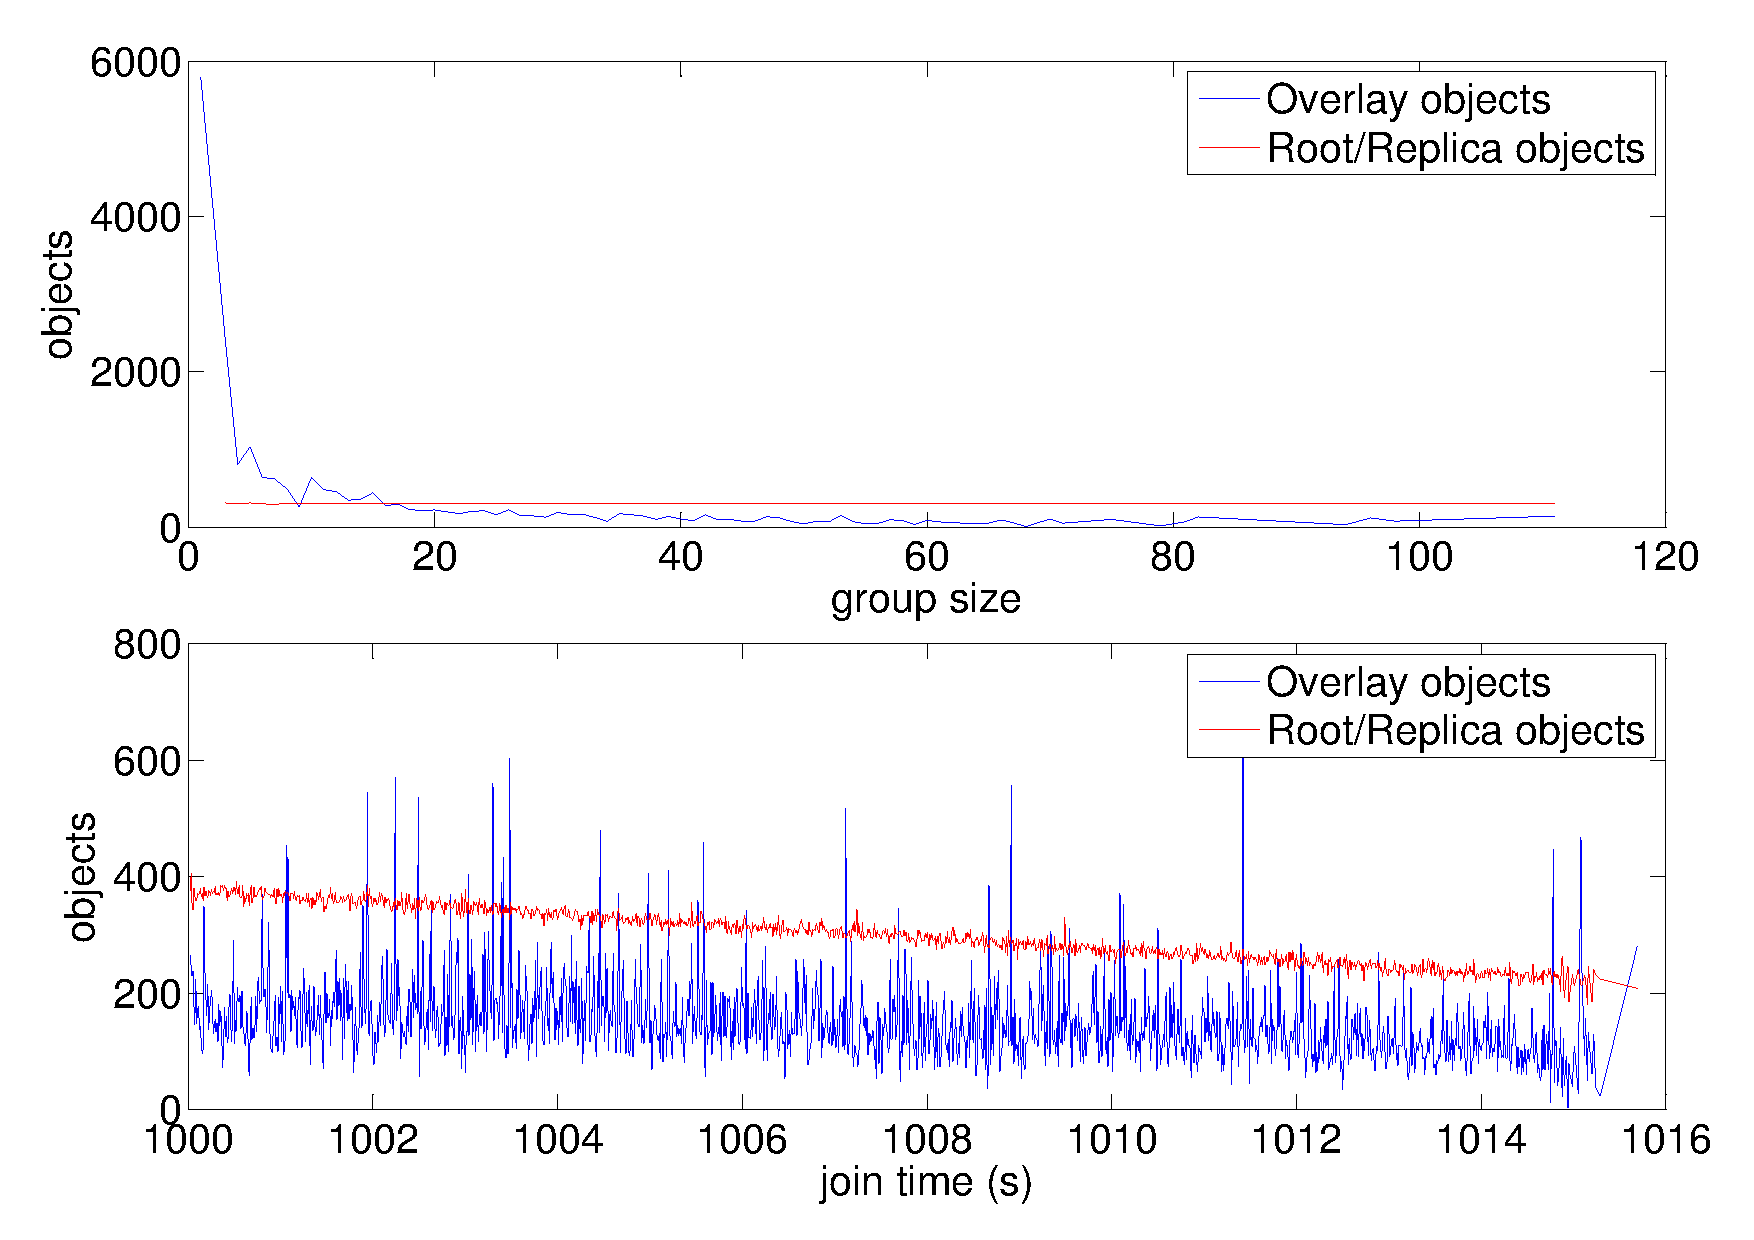
\includegraphics[clip=true, viewport=0.5cm 0.5cm 29cm 20.5cm, width=\columnwidth]{ObjectsByJtGs}
 \caption{Average number of overlay objects stored by group size and join time}
 \label{fig_objects_by_groupsize_jointime}
\end{figure}
%
Figure \ref{fig_objects_by_groupsize_jointime} (top) shows the average number of objects stored by group size. The figure shows that the number of
group objects stored in any size of group remains the same. The number of overlay objects, however, increases exponentially with a decrease in group
size. The overlay storage discrepancy can be explained by looking at how overlay objects are distributed within the network. When an overlay object
is stored, any group can be chosen and the object is then stored on a node within that group. If there are two groups that are chosen an equal number
of times, but the one group contains less nodes, each node in that group will have to store more data.

Group storage functions somewhat differently. Because every node in the simulations generates the same amount of data, smaller groups have less nodes
to store data on, but these groups also generate less data, therefore the ratio remains constant.

%\begin{figure}[htbp]
% \centering
% 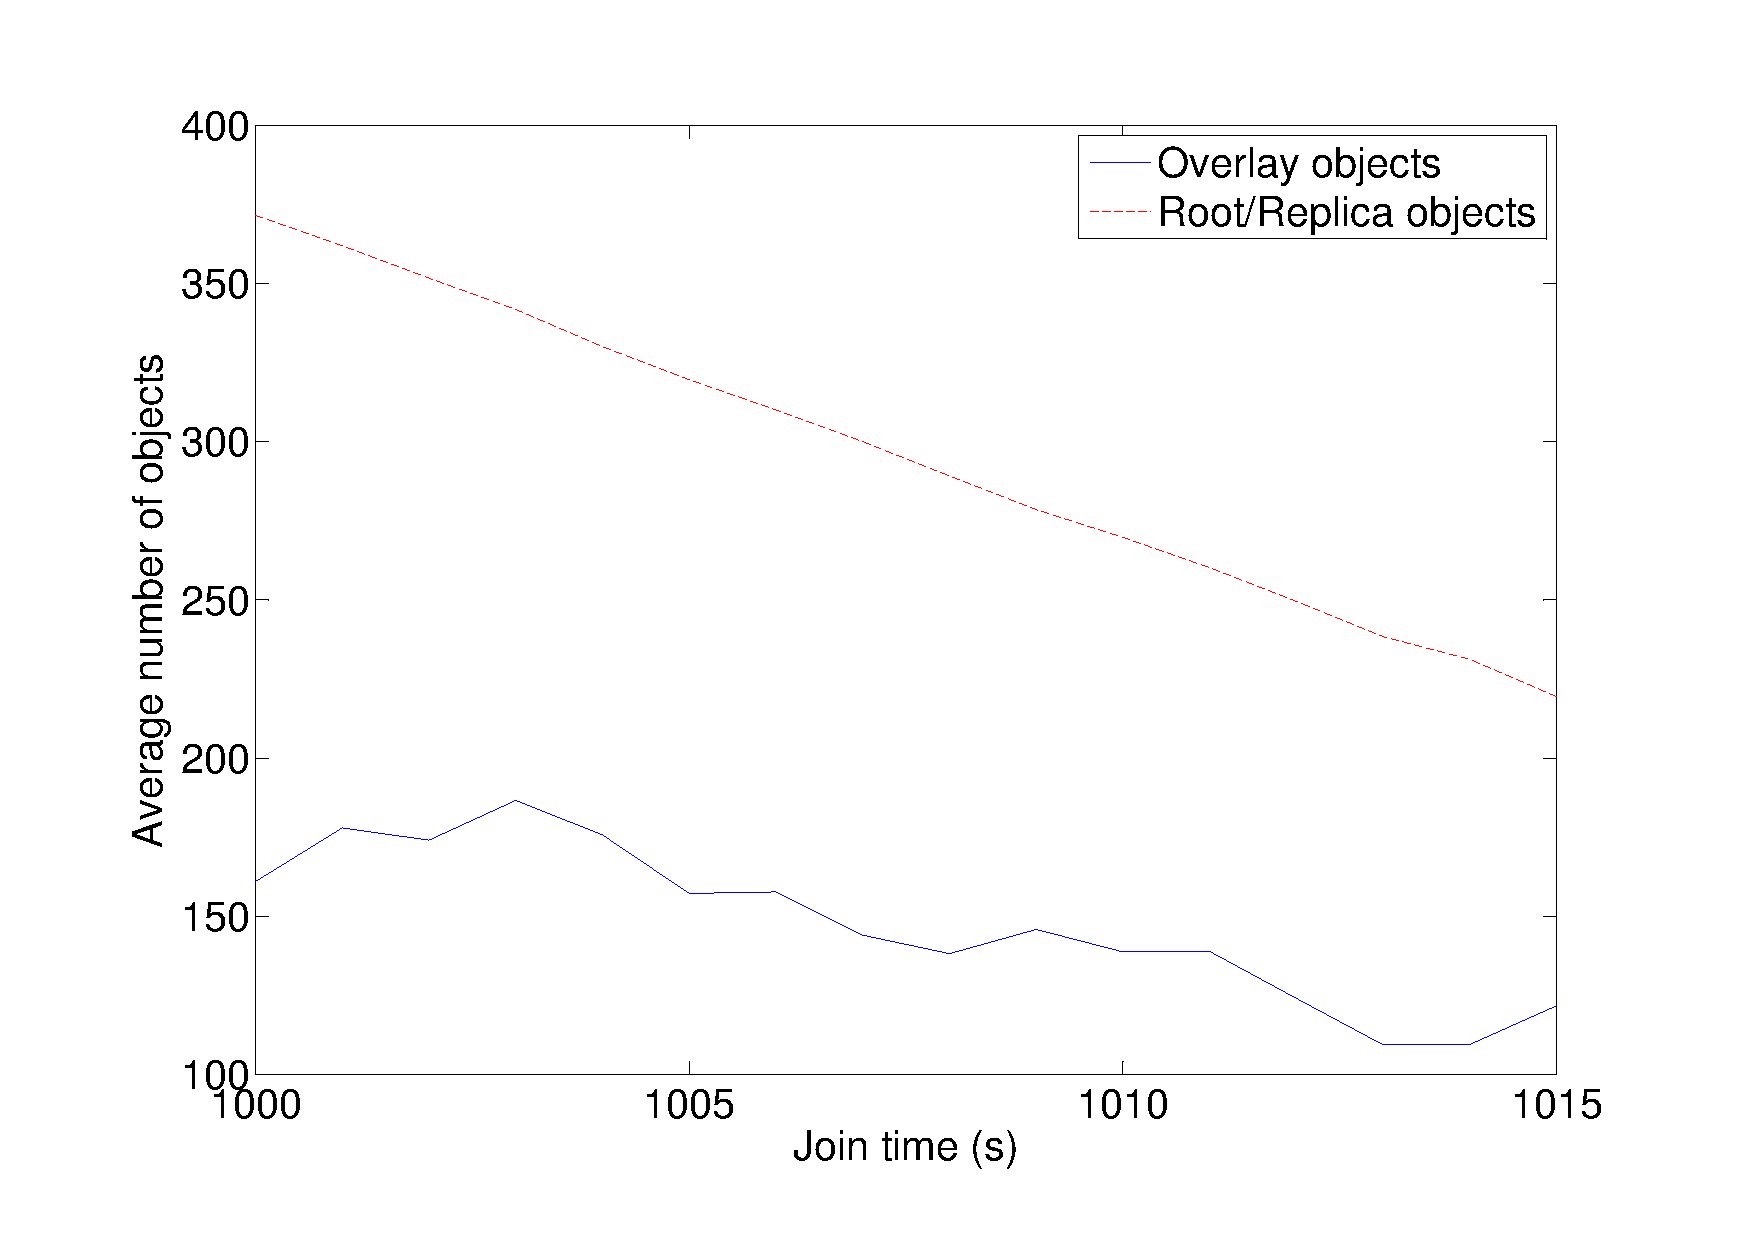
\includegraphics[clip=true, viewport=2cm 1cm 27.5cm 19.5cm, width=\columnwidth]{ObjectsByJoinTime}
% \caption{Average number of overlay objects stored by join time}
% \label{fig_objects_by_jointime}
%\end{figure}
%
Figure \ref{fig_objects_by_groupsize_jointime} (bottom) shows the average number of objects stored by join time. Join time is defined as the time at
which a certain node joined another non-empty group or the time when the joined group contained more than one node. From this figure it is evident
that nodes that have existed in the network for a longer period of time store more root and replica objects. With overlay objects, only a slight
decrease over time is perceived with a much greater variance present in the data.

For the number of root and replica objects stored on a node to decrease over time makes sense, since nodes that have been in the network longer would
have been requested to store more data. Why the number of overlay objects do not follow this pattern is thought to be as a result of how the Pastry
key space functions. When more overlay objects are added to the network, the amount of key space covered by the older nodes decrease, which means
that the number of requests that older nodes are required to serve also decreases over time and reduces the effect seen in root and replica storage.

\section{Conclusion}
\label{conclusion}

\subsection{Summary}

\subsection{Future work}

%Complete implementation
%Reliability and security
%Driver data

%\newpage
% use section* for acknowledgement
\ifCLASSOPTIONcompsoc
  % The Computer Society usually uses the plural form
  \section*{Acknowledgments}
\else
  % regular IEEE prefers the singular form
  \section*{Acknowledgment}
\fi

The financial assistance of MIH and the National Research Foundation (NRF) towards this research is hereby acknowledged. Opinions expressed and
conclusions arrived at, are those of the author and are not necessarily to be attributed to MIH or the NRF.

%\newpage
%\IEEEtriggeratref{43} %Balance the bibliography
\bibliographystyle{IEEEtran}
\bibliography{../BibTeX/P2P_MMOG}

% that's all folks
\end{document}
